%! Author = nico
%! Date = 17.06.22
\documentclass[a4paper, landscape, 8pt]{scrartcl}

% import template
% use german language
\usepackage[T1]{fontenc}
\usepackage[utf8]{inputenc}
\usepackage[english, ngerman]{babel}
\usepackage{lmodern}

% format
\usepackage{geometry}
\geometry{top=1.2cm, left=0.4cm, right=0.4cm}
\textheight = 550pt

% author
\usepackage{authblk}

% tables / tabular
\usepackage{tabularx}

% math
\usepackage{amsmath}
\usepackage{amssymb}
\usepackage{amsfonts}
\usepackage{enumitem}

% graphic
\usepackage{graphicx}

% multi column
\usepackage{multicol}

%compact items
\setlist{topsep=0pt, leftmargin=4mm, nolistsep}
\setlength{\parindent}{0cm}

% header and footer
\usepackage{fancyhdr}
\pagestyle{fancy}

% header
\fancyhead[RO]{\AUTHOR | \INSTITUTE}
\fancyhead[LO]{\TITLE}

% footer
\fancyfoot[RO]{\CREATED}

\renewcommand\headrulewidth{0pt}
\renewcommand\footrulewidth{0pt}
\headsep = -2pt
\footskip = 0pt

% define Section format
\usepackage{sectsty}
\usepackage{titlesec}
\usepackage[dvipsnames]{xcolor}

\titleformat{name=\section}[block]{\sffamily\normalsize}{}{0pt}{\colorsection}
\titlespacing*{\section}{0pt}{0pt}{0pt}
\newcommand{\colorsection}[1]{%
	\colorbox{sectioncolor!80}{\parbox{0.98\linewidth}{\vspace{-1pt}\color{white}\ #1 \vspace{-2pt}}}}

% define Subsection format
\titleformat{name=\subsection}[block]{\sffamily\small}{}{0pt}{\colorsubsection}
\titlespacing*{\subsection}{0pt}{0pt}{0pt}
\newcommand{\colorsubsection}[1]{%
	\colorbox{subsectioncolor!80}{\parbox{0.98\linewidth}{\vspace{-1pt}\color{white}\ #1 \vspace{-2pt}}}}

% define SubSubsection format
\titleformat{name=\subsubsection}[block]{\sffamily\small}{}{0pt}{\colorsubsubsection}
\titlespacing*{\subsubsection}{0pt}{0pt}{0pt}
\newcommand{\colorsubsubsection}[1]{%
	\colorbox{subsubsectioncolor!60}{\parbox{0.98\linewidth}{\vspace{-1pt}\color{white}\ #1 \vspace{-2pt}}}}


% define colors
\definecolor{sectioncolor}{HTML}{191919}
\definecolor{subsectioncolor}{HTML}{8c195f}
\definecolor{subsubsectioncolor}{HTML}{d72864}

\definecolor{b}{RGB}{0, 115, 192 } %Default highlight color
\definecolor{p}{RGB}{0, 43, 54} %Dark page color
\definecolor{t}{RGB}{131, 148, 150} %Dark text color

\definecolor{darkgreen}{RGB}{0,150,0}
\definecolor{dkgreen}{rgb}{0,0.6,0}
\definecolor{gray}{rgb}{0.5,0.5,0.5}
\definecolor{mauve}{rgb}{0.58,0,0.82}
\definecolor{DarkPurple}{rgb}{0.4, 0.1, 0.4}
\definecolor{DarkCyan}{rgb}{0.0, 0.5, 0.4}
\definecolor{LightLime}{rgb}{0.3, 0.5, 0.4}
\definecolor{Blue}{rgb}{0.0, 0.0, 1.0}
\definecolor{h}{RGB}{1, 101, 163}

% code listings
\usepackage{listings}
\usepackage{color}
\usepackage{beramono}
\usepackage{hyperref}
\hypersetup{
    colorlinks,
    linkcolor={black},
    citecolor={blue!50!black},
    urlcolor={blue!80!black}
}

\definecolor{bluekeywords}{rgb}{0,0,1}
\definecolor{greencomments}{rgb}{0,0.5,0}
\definecolor{redstrings}{rgb}{0.64,0.08,0.08}
\definecolor{xmlcomments}{rgb}{0.5,0.5,0.5}
\definecolor{types}{rgb}{0.17,0.57,0.68}

\lstdefinestyle{eclipse-style}{
	language=Java,
	showstringspaces=false,
	basicstyle=\ttfamily\scriptsize,
	keywordstyle=\color{RoyalBlue}\ttfamily,
    stringstyle=\color{darkgreen}\ttfamily,
	commentstyle=\color{DarkPurple!60}\ttfamily,
	identifierstyle=\color{black}\ttfamily,
	escapeinside={£}{£}, % latex scope within code
	breaklines=true,
	breakatwhitespace=true,
	showspaces=false,
	showtabs=false,
	tabsize=2,
	morekeywords={length},
	numberstyle=\tiny\color{black},
	aboveskip = 0em,
	belowskip = 0em,
	xleftmargin= 0em,
	framexleftmargin= 0em,
	gobble=20
}
\lstset{
	style=eclipse-style
	% literate=  % Allow for German characters in lstlistings.
	% {Ö}{{\"O}}1
	% {Ä}{{\"A}}1
	% {Ü}{{\"U}}1
	% {ü}{{\"u}}1
	% {ä}{{\"a}}1
	% {ö}{{\"o}}1}
}

% creation date
\usepackage{filemod}
\newcommand{\CREATED}{\filemodprintdate{\jobname}}

% front page
\newcommand{\AUTHOR}{Nico Fehr }
\newcommand{\INSTITUTE}{Ostschweizer Fachhochschule}

% no indentation
\setlength{\parindent}{0cm}

% document information
\newcommand{\SUBJECT}{}
\newcommand{\TITLE}{Cheat sheet für OOP2}

% document content
\begin{document}

    \begin{multicols*}{4}
        \setlength{\columnseprule}{0.4pt}
        \footnotesize

        \section{Generics}
            \subsection{Terminologie}
                \textcolor{subsectioncolor}{Generische Klasse}
                \newline
                Klasse mit \textcolor{subsectioncolor}{generischen Parametern}
                \begin{lstlisting}
                    class Stack<T> {
                    // ...
                    }
                \end{lstlisting}

                \textcolor{subsectioncolor}{Generischer Typ}
                \newline
                Klasse die mit \textcolor{subsectioncolor}{konkretem Typ} instanziiert wird.
                \begin{lstlisting}
                    Stack<String> stack1;
                    Stack<Integer> stack2;
                    Stack<Person> stack3;
                    Stack<double[]> stack4;
                    Stack<Object> stack5;
                \end{lstlisting}
                \begin{itemize}
                    \item Kann ein statisches Attribut generisch sein?
                    \item \begin{lstlisting}
                    public class MobileDevice<T> {
                        private static T os;
                        //..
                    }
                    \end{lstlisting}
                    \begin{itemize}
                        \item {\bfseries Nein}
                        \begin{itemize}
                            \item Statisches Attribut wird zwischen Instanzen geteilt
                            \item Wäre unklar, welchen Typ das statische Attribut tatsächlich hat
                        \end{itemize}
                    \end{itemize}
                \end{itemize}

            \subsection{Generische Klassen}
                \textcolor{subsectioncolor}{Typ-Parameter}
                \newline
                Platzhalter für generischen Typ
                \begin{lstlisting}
                    <T>
                \end{lstlisting}

                \textcolor{subsectioncolor}{Typ-Argument}
                \newline
                Typ bei Einsatz angeben
                \begin{lstlisting}
                    Stack<String> stack1;
                    Stack<Integer> stack2;
                \end{lstlisting}

            \subsection{Generische Methoden}
                \begin{itemize}
                    \item Typ-Variable innerhalb spezifischer Methode
                    \item Aufrufer bestimmt Typ-Argument
                \end{itemize}
                \begin{lstlisting}
                    public <E> Stack<E> multiPush(E value, int times) {
                        var result = new Stack<E>();
                        ...
                \end{lstlisting}

        \section{Listen und Arrays}
            \subsection{Arrays}
                \begin{itemize}
                    \item Speichern gleichartige Objekte (Elemente)
                    \item Zugriff über Index
                    \item {\bfseries Arrays speichern Referenzen auf Objekte} $\to$ ändert sich referenziertes Objekt,
                    so ändert sich Inhalt des Arrays
                \end{itemize}
        
                \subsubsection{Arrays im Speicher}
                    Array wächst $\to$ muss in neuen Block kopiert werden (neue Grösse [*1.5 Java-Standard])
                    \newline
                    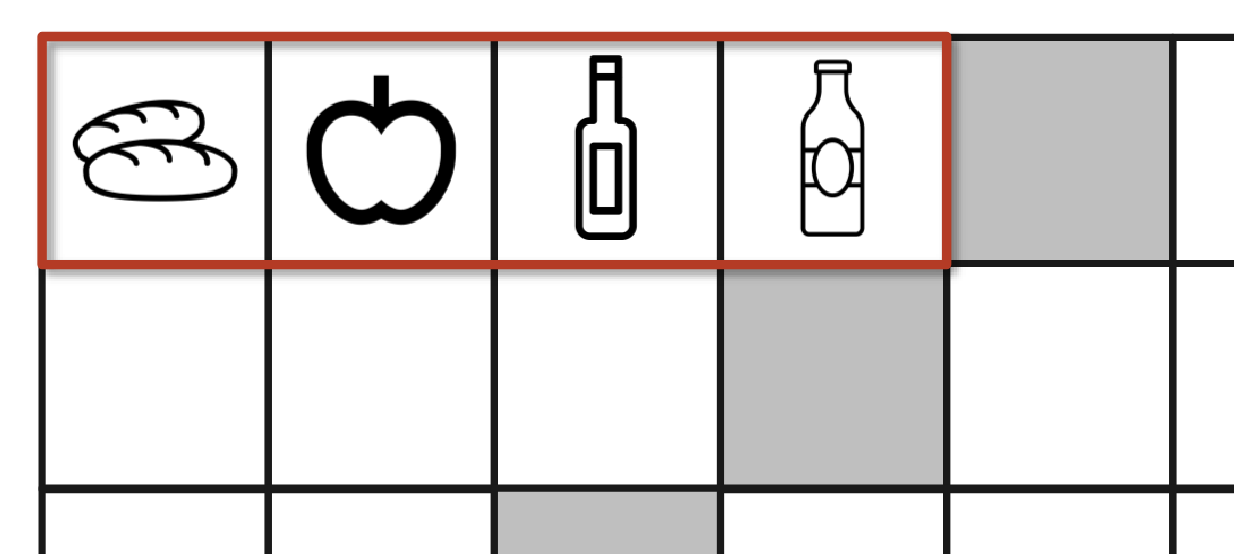
\includegraphics[scale=0.13]{graphic/00_array_im_speicher}
        
                \subsubsection{LinkedList im Speicher}
                    \begin{tabular}{l | r}
                        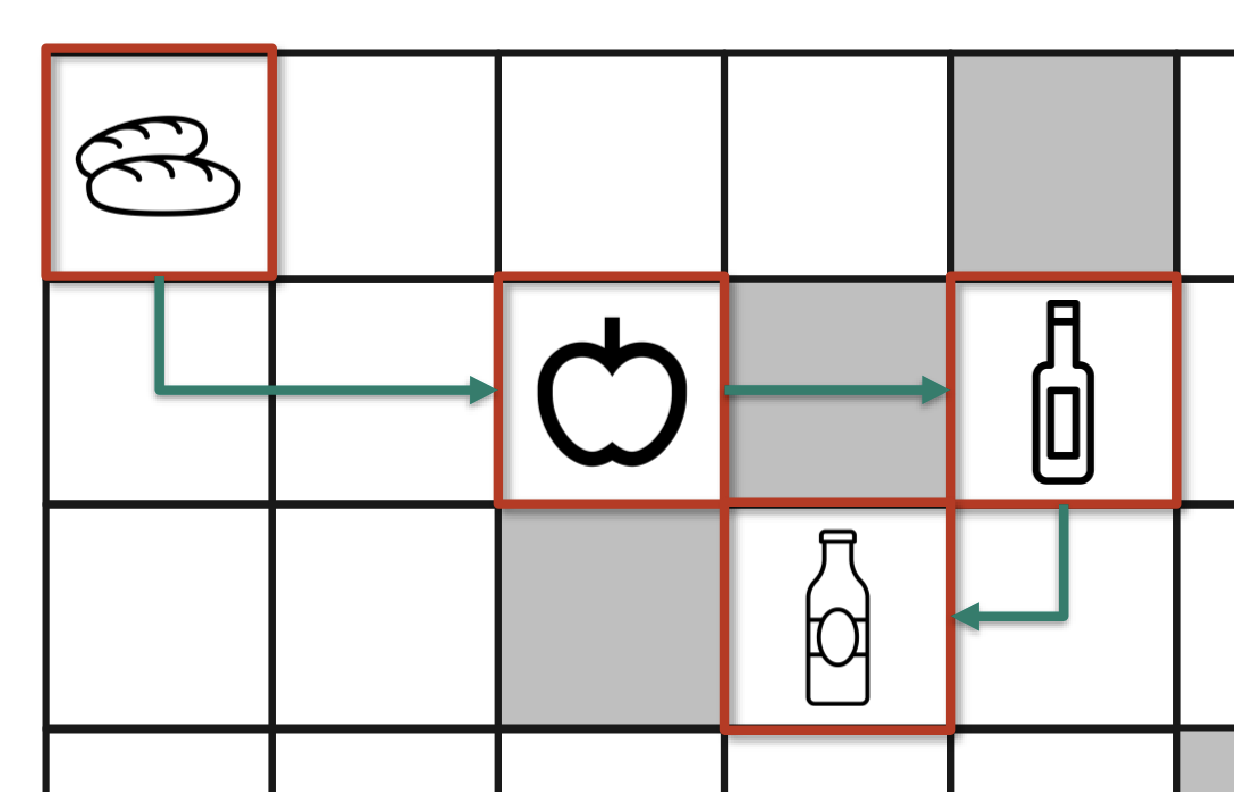
\includegraphics[scale=0.13]{graphic/01_linkedlist_im_speicher} &
                        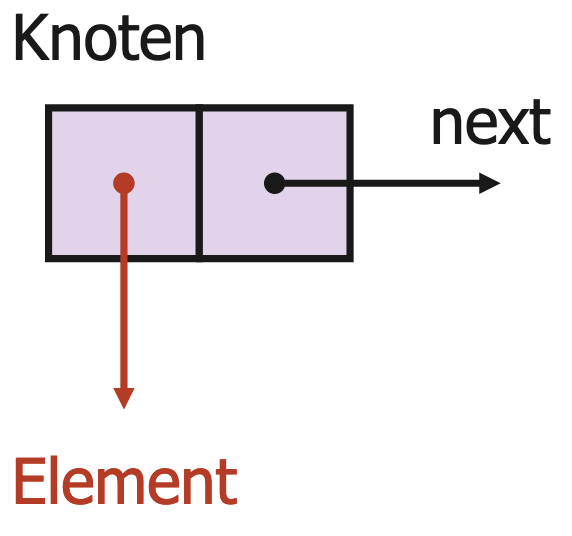
\includegraphics[scale=0.14]{graphic/07_knoten_linkedlist} \\
                    \end{tabular}

            \subsection{Auswahl Datenstruktur}
                Wovon kann die Wahl abhängig gemacht werden? $\to$ Laufzeiten von verschiedenen Use-Cases betrachten
                \newline
                \textcolor{subsectioncolor}{Laufzeiten-Vergleich}
                \newline
                \begin{tabular}{ |c|c|c| }
                    \hline
                    & {\bfseries Lesen} & {\bfseries Element einfügen} \\
                    \hline
                    {\bfseries Array} & $O(1)$ & $O(n)$ \\
                    {\bfseries Liste} & $O(n)$ & $O(1)$ \\
                    \hline
                \end{tabular}

        \section{Algorithmenparadigmen}
            {\bfseries Algorithmus: Präzise endliche Beschreibung eines allgemeinen Verfahrens unter Verwendung
            ausführbarer elementarer Schritte}

            \subsection{Backtracking}
                \begin{itemize}
                    \item Konzept:
                    \begin{itemize}
                        \item Trial \& Error
                        \item Aktueller Zweig führt nicht zur Lösung:
                        \begin{itemize}
                            \item Zurück zur letzten Entscheidung (Backtracking)
                            \item Anderen Pfad probieren
                        \end{itemize}
                    \end{itemize}
                \end{itemize}
                \textcolor{subsectioncolor}{Implementierung Pseudocode}
                \begin{enumerate}
                    \item Ziel erreicht:
                    \begin{enumerate}
                        \item Lösungspfad aktualisieren
                        \item True zurückgeben
                    \end{enumerate}
                    \item Wenn (x, y) bereits Teil des Lösungspfades
                    \begin{enumerate}
                        \item False zurückgeben
                    \end{enumerate}
                    \item (x, y) als Teil des Lösungspfades markieren
                    \item In X-Richtung suchen: →
                    \item Keine Lösung: In Y-Richtung abwärts suchen: ↓
                    \item Keine Lösung: Zurück in X-Richtung suchen: ←
                    \item Keine Lösung: Aufwärts in Y-Richtung suchen: ↑
                    \item Immer noch keine Lösung: (x, y) aus Lösungspfad entfernen // Backtracking
                    \item False zurückgeben
                \end{enumerate}

                \subsubsection{Cookbook}
                    \begin{enumerate}
                        \item Position auf Feld (Schachbrett/Labyrinth) markieren
                        \item Rekursionsabbruch (z.B.\ alle Felder besucht, Ausgang gefunden)
                        \begin{itemize}
                            \item \texttt{return true;}
                        \end{itemize}
                        \item Alle Optionen probieren
                        \begin{enumerate}
                            \item Neues Feld / Koordinate festlegen
                            \item Überprüfen ob Feld gültig ist \& noch nicht besucht wurde
                            \begin{enumerate}
                                \item Wenn ja $\to$ prüfen ob rekursiver Aufruf \texttt{true} zurückgibt
                                \begin{enumerate}
                                    \item Wenn ja $\to$ \texttt{return true;}
                                \end{enumerate}
                            \end{enumerate}
                        \end{enumerate}
                        \item Backtracking: Markierung von Feld entfernen \& \texttt{return false;}
                    \end{enumerate}

                %\subsubsection{Labyrinth}

                \subsubsection{Knights-Tour}
                    \begin{enumerate}
                        \item Feld markieren
                        \item Abbruchsbedinung: Position so gross wie Anzahl Felder $\to$ Alle Felder besucht
                        \item Alle möglichen Züge mit Springer probieren und neue (X|Y) berechnen
                        \item Überprüfen ob neues Feld innerhalb des Spielbretts \& ob Feld noch nicht besucht
                        \item Überprüfen ob rekursiver Aufruf Abbruchsbedingung erreicht. Wenn ja: \texttt{return true;}
                        \item Falls beide Bedingungen (4, 5) nicht erfüllt sind $\to$ Markierung von Feld entfernen
                        und mit \texttt{return true;} backtracken
                    \end{enumerate}
                    \textcolor{subsectioncolor}{Java}
                    \begin{lstlisting}
                    public static boolean knightTour(int[][] visited, int x, int y, int pos) {
                        visited[x][y] = pos;

                        if (pos >= N * N) {
                            return true;
                        }
                        for (int k = 0; k < 8; k++) {
                            int newX = x + row[k];
                            int newY = y + col[k];

                            if (isValid(newX, newY) && visited[newX][newY] == 0) {
                                if (knightTour(visited, newX, newY, pos+1)) {
                                    return true;
                                }
                            }
                        }

                        visited[x][y] = 0;
                        return false;
                    }

                    private static boolean isValid(int x, int y) {
                        return x >= 0 && y >= 0 && x < N && y < N;
                    }
                    \end{lstlisting}

            \subsection{Rekursion}
                \begin{itemize}
                    \item Rekursionsabbruch (Base Case)
                    \begin{itemize}
                        \item mindestens 1 base case
                        \item Rekursive Kette muss base case erreichen (abbrechen)
                    \end{itemize}
                    \item Ausführung bewegt sich Richtung base case
                \end{itemize}

                \subsubsection{NDigitNums}
                    \begin{lstlisting}
                    public static void findNDigitNums(String currentNumber, int n, int target, List<Integer>
                        resultList) {
                        if (n > 0 && target >= 0) {
                            char digit = '0';
                            if (currentNumber.equals("")) {
                                digit = '1';
                            }
                            while (digit <= '9') {
                                String num = currentNumber + digit;
                                int newTarget = target - (digit - '0');
                                findNdigitNums(num, n-1, newTarget, resultList);
                                digit++;
                            }
                        } else if (n == 0 && target == 0) {
                            resultList.add(Integer.valueOf(currentNumber));
                        }
                    }
                    \end{lstlisting}
        
                \subsubsection{Fakultät}
                    \textcolor{subsectioncolor}{Funktion}
                    \newline
                    f(n) =
                    \begin{cases}
                        1 & if \; n=0 \\
                        n \cdot f(n-1) & else
                    \end{cases}
                    \newline

                    \textcolor{subsectioncolor}{Java Beispiel}
                    \begin{lstlisting}
                    static int recursiveFactorial(int n) {
                        if (n == 0)
                            return 1;
                        else
                            return n * recursiveFactorial(n-1);
                    }
                    \end{lstlisting}

                \subsubsection{Endrekursion}
                    Wenn linear rekursive Methode als {\bfseries letzten Schritt} rekursiven Aufruf ausführt
                    \begin{itemize}
                        \item können leicht in nicht-rekursive Algorithmen umgewandelt werden
                        \item nicht-rekursive Algorithmen benötigen meist weniger Ressourcen
                    \end{itemize}
                    \newline
                    \textcolor{subsectioncolor}{Java Beispiel}
                    \begin{lstlisting}
                    private static int tailrecsum(int x, int total) {
                        if (x == 0)
                            return total;
                        else
                            return tailrecsum(x-1, total+x);
                    }
                    \end{lstlisting}

            \subsection{Greedy}
                \begin{itemize}
                    \item Konzept: Es soll bestimmte Eigenschaft minimiert / maximiert werden
                    \item Ansatz:
                    \begin{itemize}
                        \item in jedem Teilschritt {\bfseries möglichst viel} erreichen
                        \item in jedem Teilschritt {\bfseries möglichst optimale} Lösung wählen
                    \end{itemize}
                \end{itemize}
                \subsubsection{Rückgeld Beispiel}
                    \begin{itemize}
                        \item Preis: 7 CHF
                        \item Bezahlt mit: 15 CHF
                        \item Ziel: Rückgeld mit minimaler Anzahl Münzen
                        \item Vorgehen:
                        \begin{itemize}
                            \item Nehme grösste Münze unter Zielwert und ziehe sie von diesem ab
                            \item Verfahre bis Zielwert = 0
                        \end{itemize}
                    \end{itemize}

                \subsubsection{Set-Covering Problem}
                    \textcolor{subsectioncolor}{Beispiel Abdeckung Radiostationen in den USA}
                    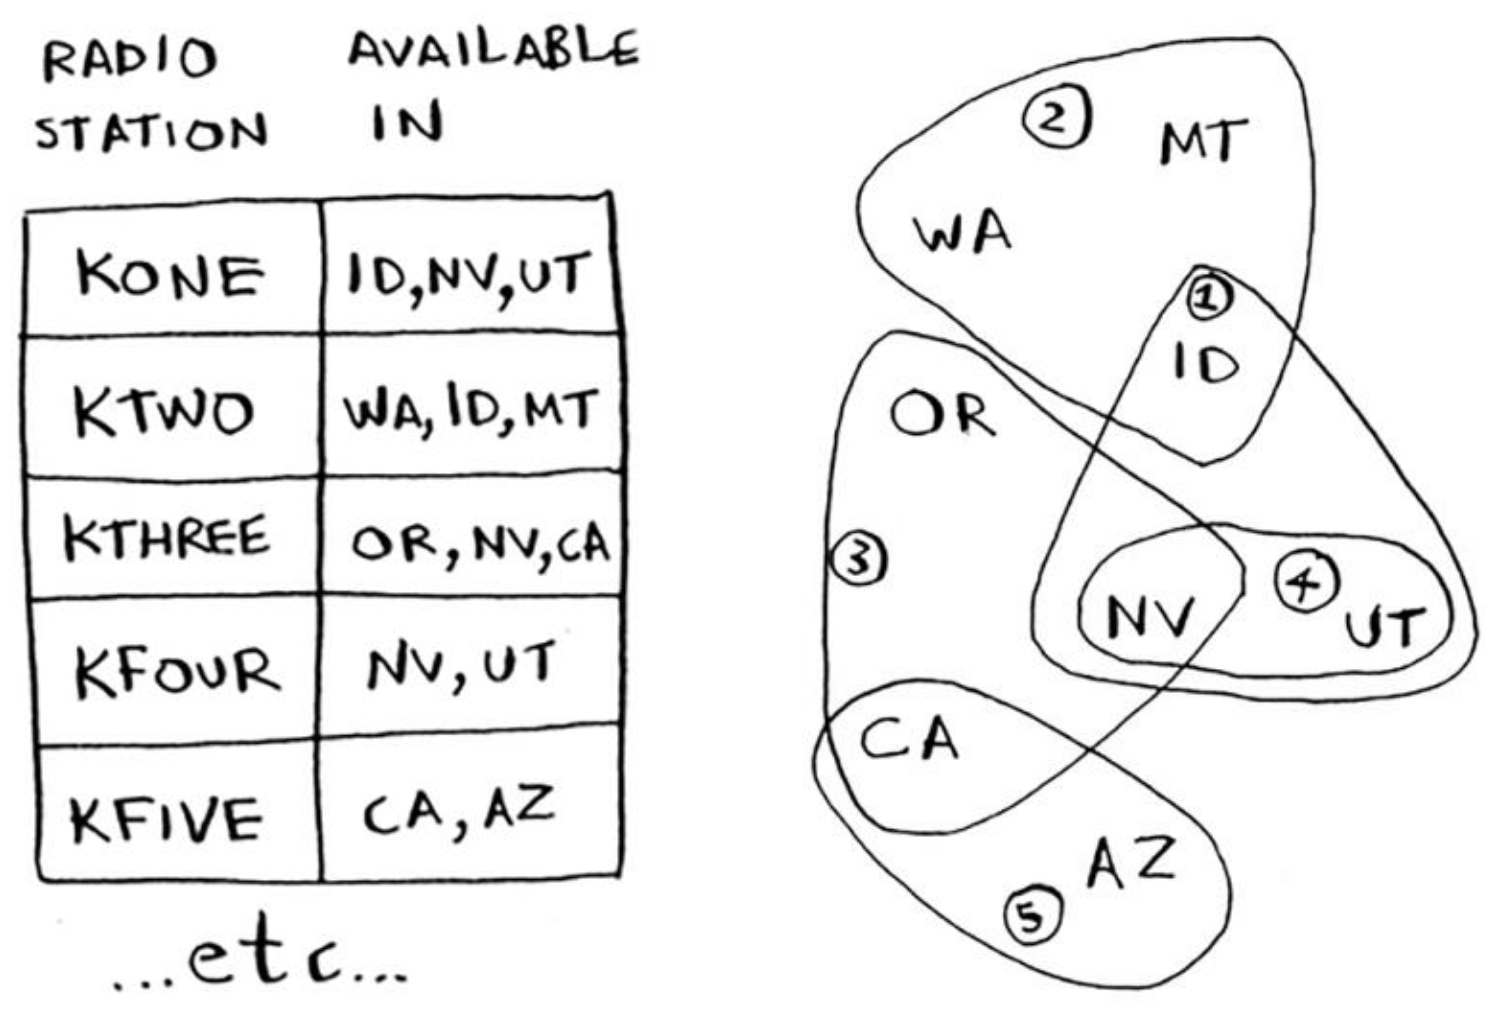
\includegraphics[scale=0.15]{graphic/08_set_covering_radio_stations}
                    \begin{itemize}
                        \item Optimaler Algorithmus
                        \begin{itemize}
                            \item Alle Teilmengen der Stationen aufzählen
                            \item Minimale Anzahl Stationen wählen
                            \item {\bfseries Problem:} $2^n$ mögliche Kombinationen (Potenzmenge)
                        \end{itemize}
                    \end{itemize}
                    {\bfseries $\to$ Es gibt keinen Algorithmus, der Problem schnell genug löst}
                    \newline
                    \textcolor{subsectioncolor}{Alternative}
                    \begin{itemize}
                        \item Wähle Sender, der meisten Sender abdeckt, die noch nicht abgedeckt sind
                        \item Widerholen, bis alle Sender abgedeckt sind
                    \end{itemize}
                    \begin{lstlisting}
                    public static void calculateSolution(HashSet<String> statesNeeded, HashMap<String, HashSet<String>> stations) {
                        var finalStations = new HashSet<String>();
                        while (!statesNeeded.isEmpty()) {
                            String bestStation = "";
                            var statesCovered = new HashSet<String>();
                            for (String station : stations.keySet()) {
                                var covered = new HashSet<String>(statesNeeded);
                                covered.retainAll(stations.get(station));
                                if (covered.size() > statesCovered.size()) {
                                    bestStation = station;
                                    statesCovered = covered;
                                }
                            }
                            statesNeeded.removeAll(statesCovered);
                            finalStations.add(bestStation);
                        }
                        System.out.println(finalStations);
                    }
                    \end{lstlisting}

            \subsection{Divide-and-Conquer / Teile-und-Herrsche}
                \begin{itemize}
                    \item Problem aufteilen
                    \item Kleinere Probleme lösen
                    \item Rekursive Rückführung des Problems auf identisches mit kleinerer Eingabemenge
                \end{itemize}

                \subsubsection{Binärsuche}
                \textcolor{subsectioncolor}{Iterative Implementierung}
                \begin{lstlisting}
                    public static void searchBinary(int[] intArr, int start, int end, int searchElement) {
                        int pivot = start + ((end - start) / 2);
                        if (intArr.length == 0) {
                            System.out.println("Array leer.");
                            return;
                        }
                        if (pivot >= intArr.length){
                            System.out.println(searchElement + " nicht im Array enthalten.");
                            return;
                        }
                        if (searchElement > intArr[pivot]) {
                            System.out.println(start + " " + end + " " + pivot);
                            searchBinary(intArr, pivot + 1, end, searchElement);
                        } else if (searchElement < intArr[pivot] && start != pivot) {
                            searchBinary(intArr, start, pivot - 1, searchElement);
                        } else if(searchElement == intArr[pivot]) {
                            System.out.println(searchElement + " an Position " + pivot + " enthalten.");
                        } else{
                            System.out.println(searchElement + " nicht im Array enthalten.");
                        }
                    }
                \end{lstlisting}
                \textcolor{subsectioncolor}{Rekursive Implementierung}
                \begin{lstlisting}
                    int binarySearch(int array[], int x, int low, int high) {
                        if (high >= low) {
                            int mid = low + (high - low) / 2;
                            if (array[mid] == x) // Wenn Element gefunden: zurueckgeben
                                return mid;
                            if (array[mid] > x) // In der linken Haelfte suchen
                                return binarySearch(array, x, low, mid - 1);
                            return binarySearch(array, x, mid + 1, high); // In der rechten Haelfte suchen
                        }
                        return -1;
                    }
                \end{lstlisting}

                \subsubsection{Mergesort}
                    $\to$ siehe Sortieralgorithmen $\to$ Mergesort

            \subsection{Dynamische Programmierung}
            \textcolor{subsectioncolor}{Fibonacci Beispiel {\bfseries Iterativ}}
            \begin{lstlisting}
                    static void fibonacciIterativ(int n) {
                        int num1 = 0
                        int num2 = 1;
                        int counter = 0;

                        while (counter < n) {
                            System.out.print(num1 + " ");

                            int num3 = num2 + num1;
                            num1 = num2;
                            num2 = num3;
                            counter++;
                        }
                    }
            \end{lstlisting}
            \textcolor{subsectioncolor}{Fibonacci Beispiel {\bfseries Dynamisch}}
            \begin{lstlisting}
                    static int fibonacciDynamisch(int n) {
                        int f[] = new int[n + 2];

                        int i;
                        f[0] = 0;
                        f[1] = 1;

                        for (i = 2; i <= n; i++) {
                            f[i] = f[i - 1] + f[i - 2];
                        }

                        return f[n];
                    }
            \end{lstlisting}

        \section{Analyse von Algorithmen}
            \subsection{O-Notation / Big-O-Notation}
                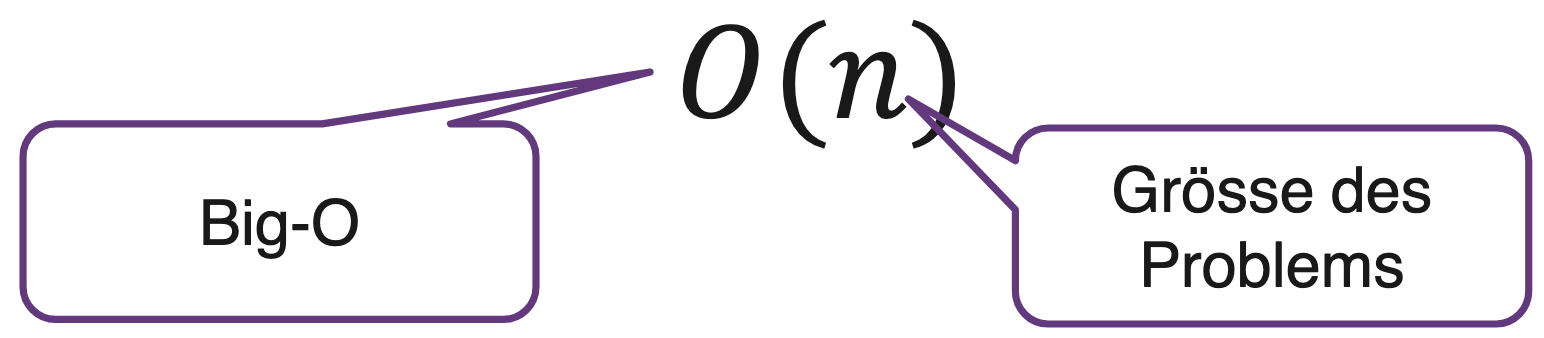
\includegraphics[scale=0.15]{graphic/15_big_o_notation_erklaerung}
                \newline
                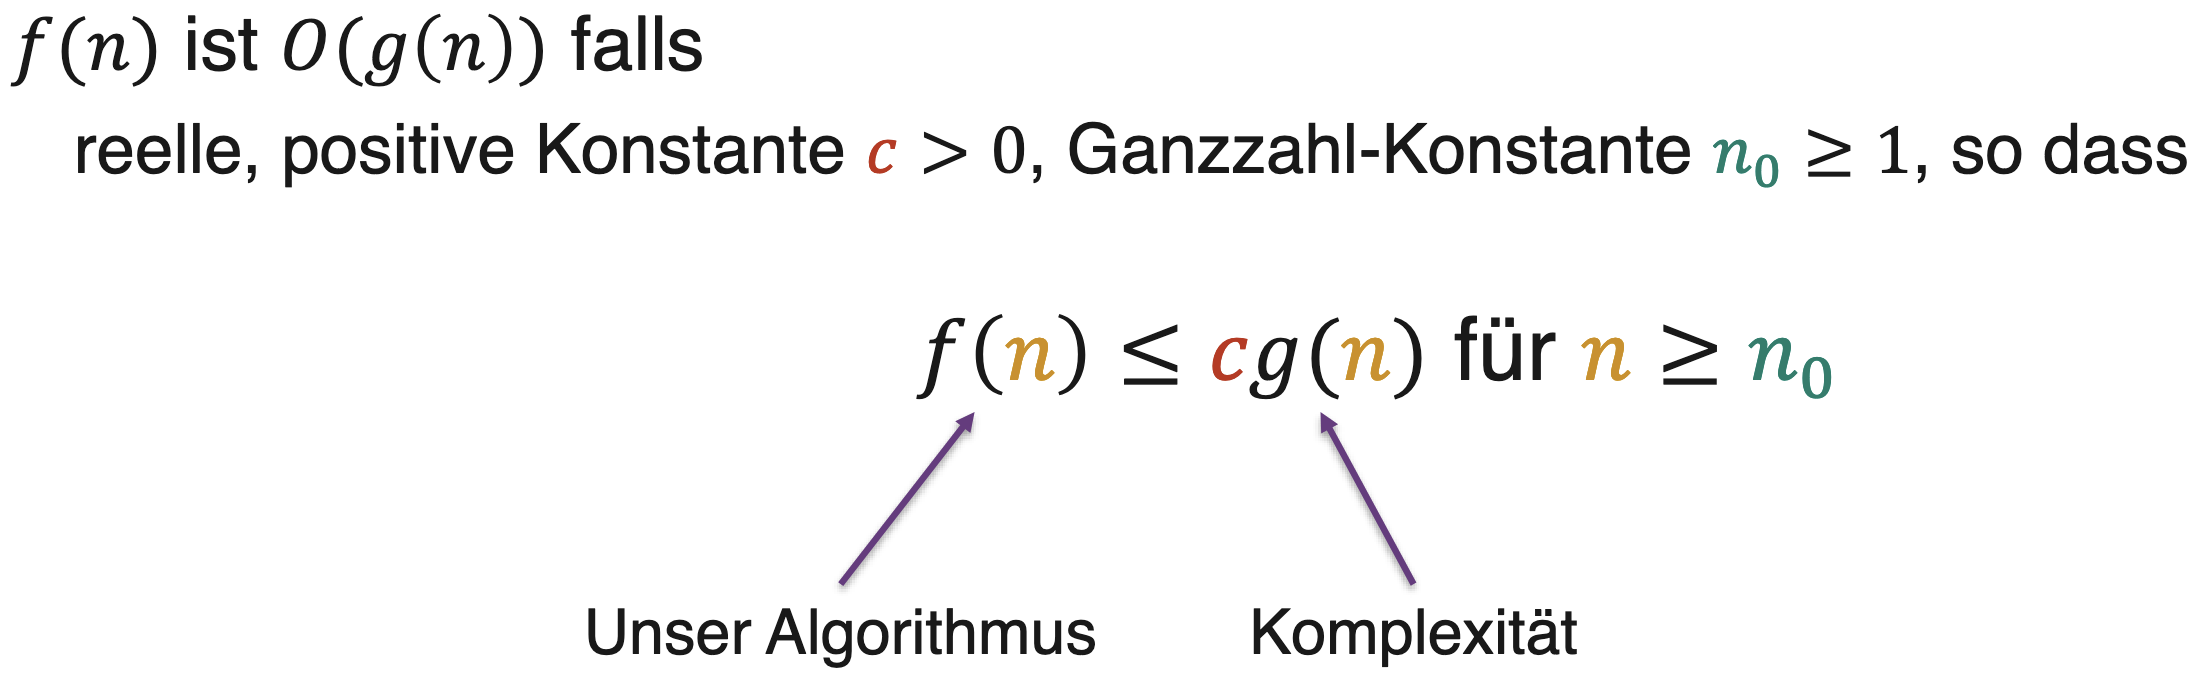
\includegraphics[scale=0.15]{graphic/14_big_o_notation_herleitung}
                \newline
                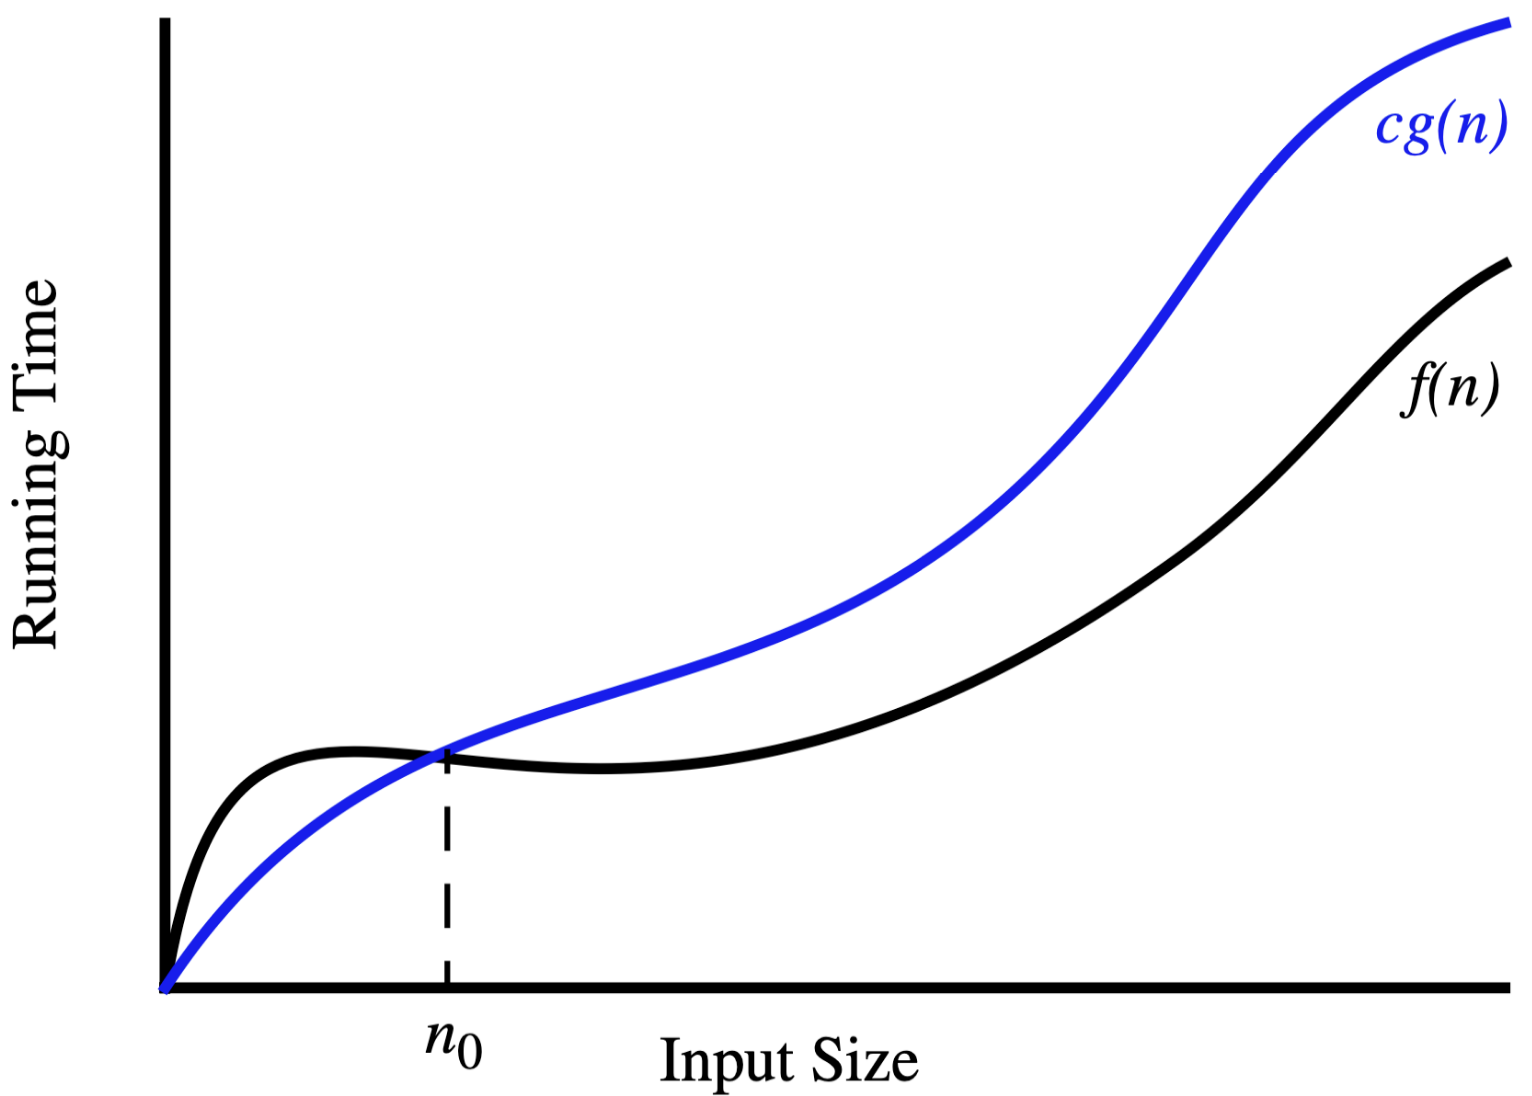
\includegraphics[scale=0.15]{graphic/03_big_o_notation}
                \begin{itemize}
                    \item Regeln
                    \begin{itemize}
                        \item Falls $f(n)$ Polynom vom Grad $d$ ist, gilt $f(n) \in O(n^d)$, d.h:
                        \begin{itemize}
                            \item Alle tieferen Potenzen weglassen
                            \item Alle Konstanten weglassen
                        \end{itemize}
                        \item Jeweils optimalste Funktion verwenden (tiefst mögliche Potenz)
                        \item So stark wie möglich vereinfachen
                        \begin{itemize}
                            \item $3n + 5$ ist $O(n)$, statt $3n + 5$ ist $O(3n)$
                        \end{itemize}
                    \end{itemize}
                    \item Häufige Funktionen
                    \begin{itemize}
                        \item konstant $\approx 1$
                        \item logarithmisch $\approx \log(n)$
                        \item linear $\approx n$
                        \item N-log-N $\approx n*\log(n)$
                        \item quadratisch $\approx n^2$
                        \item kubisch $\approx n^3$
                        \item exponentiell $\approx 2^n$
                    \end{itemize}
                    \item big-O
                    \begin{itemize}
                        \item $f(n)$ ist $O(g(n))$ falls $f(n)$ asymptomatisch {\bfseries kleiner oder gleich} $g(n)$
                        ist: $f(n) \leq cg(n)$ für $n \geq n_0$
                    \end{itemize}
                    \item big-Omega
                    \begin{itemize}
                        \item $f(n)$ ist $\Omega(g(n))$ falls $f(n)$ asymptomatisch {\bfseries grösser oder gleich}
                        $g(n)$ ist: $f(n) \geq c * g(n)$ für $n \geq n_0$
                    \end{itemize}
                    \item big-Theta
                    \begin{itemize}
                        \item $f(n)$ ist $\Theta(g(n))$ falls $f(n)$ asymptomatisch {\bfseries gleich} $g(n)$ ist:
                        $c'g(n) \leq f(n) \leq c''g(n)$ für $n \geq n_0$
                    \end{itemize}
                \end{itemize}

            \subsection{Operationen Zählen}
                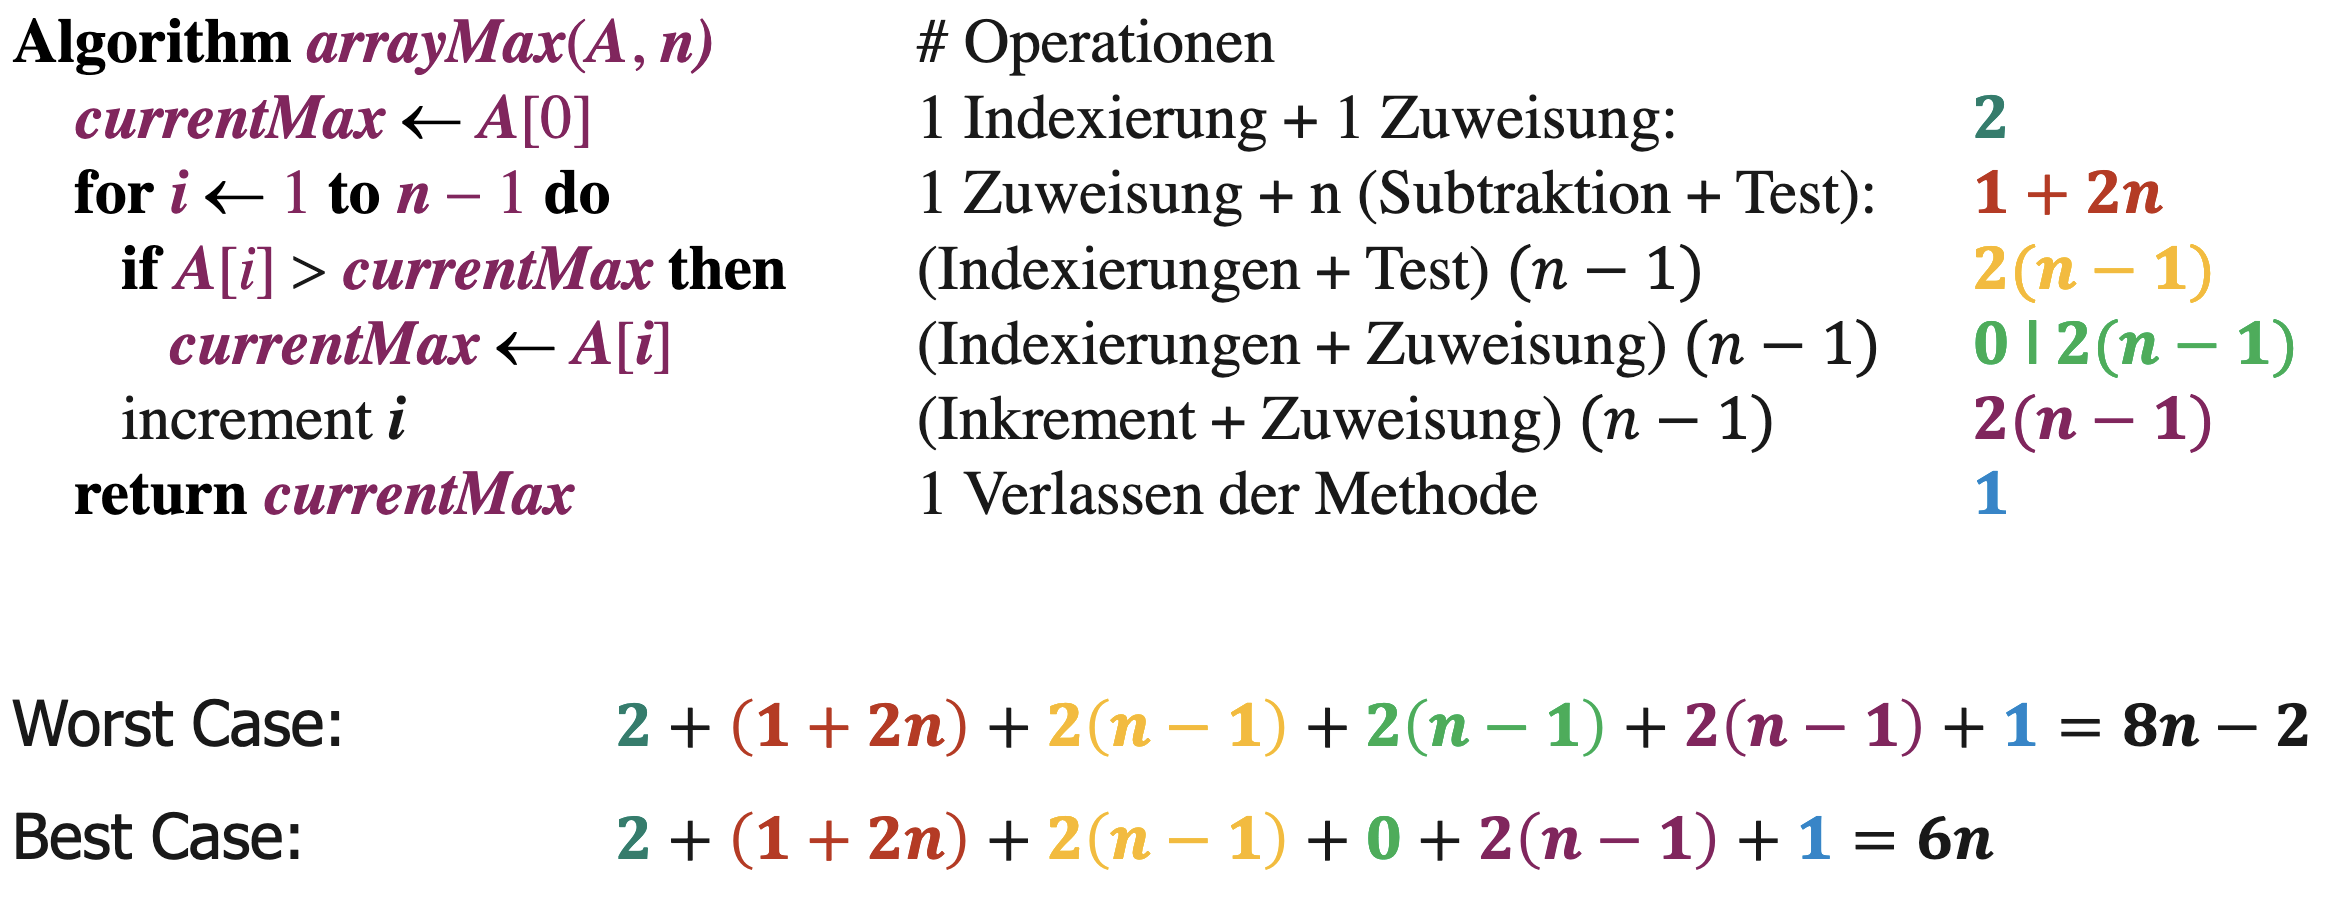
\includegraphics[scale=0.17]{graphic/04_primitive_operationen_zaehlen}

            \subsection{Empirie / Empirische Analyse}
                \textcolor{subsectioncolor}{Ablauf Empirie}
                \begin{enumerate}
                    \item Algorithmus implementieren
                    \item Algorithmus mit unterschiedlichen Eingaben ausführen
                    \item Ergebnisse aufzeichnen und vergleichen
                \end{enumerate}
                \begin{lstlisting}
                    long startTime = System.currentTimeMillis()
                    /* Algorithmus */
                    long endTime = System.currentTimeMillis();
                    long elapsed = endTime - startTime;
                \end{lstlisting}
                \textcolor{subsectioncolor}{Herausforderungen: Empirischer Vergleich von Algorithmen}
                \begin{itemize}
                    \item Datengrundlage (Testdaten) sollte repräsentativ sein
                    \item Abhängigkeiten vom System $\to$ z.B Memory, CPU-Leistung, etc.
                \end{itemize}

                Wichtig: Abgrenzung Empirische Analyse, Theoretische Analyse mit O-Notation
        
        \section{Sortieralgorithmen}
            \subsection{Bogosort}
                \begin{tabular}{|l|}
                    \hline
                    \begin{lstlisting}
                    void bogo(int[] arr) {
                        int shuffle = 1;
                        for(; !isSorted(arr); shuffle++)
                            shuffle(arr);
                    }

                    void shuffle(int[] arr) {
                        int i = arr.length - 1;
                        while (i > 0) {
                            swap (arr, i--, (int) (Math.random() * i));
                    }
                    \end{lstlisting} \\
                    \hline
                    Worst Case: $Infinite$ \\
                    Average Case: $n*n!$ \\
                    Best Case: $n$ \\
                    \hline
                \end{tabular}

            \subsection{Insertionsort}
                \begin{itemize}
                    \item Elementarer Sortieralgorithmus
                \end{itemize}
                \begin{tabular}{|l|}
                    \hline
                    \begin{lstlisting}
                    public static void sort(Comparable[] a) {
                        int n = a.length;
                        for (int i = 1; i < n; i++) {
                            for (int j = i; j > 0 && less(a[j], a[j - 1]; j--) {
                                swap(a, j, j - 1);
                            }
                        }
                    }
                    \end{lstlisting} \\
                    \hline
                    Worst Case: $O(n^2)$ \\
                    Average Case: $O(n^2)$ \\
                    Best Case: $O(n)$ \\
                    \hline
                \end{tabular}

            \subsection{Selection Sort}
                \begin{itemize}
                    \item Elementarer Sortieralgorithmus
                \end{itemize}
                \begin{tabular}{|l|}
                    \hline
                    \begin{lstlisting}
                    static void selectionSort(int[] array) {
                        int marker = array.length - 1;
                        while (marker >= 0) {
                            int max = 0;
                            for (int i = 1; i <= marker; i++) {
                                if (array[i] > array[max]) {
                                    max = i;
                                }
                            }
                            swap(array, marker, max);
                            marker--;
                        }
                    }
                    \end{lstlisting} \\
                    \hline
                    Worst Case: $O(n^2)$ \\
                    Average Case: $O(n^2)$ \\
                    Best Case: $O(n^2)$ \\
                    \hline
                \end{tabular}

            \subsection{Bubblesort}
                \begin{tabular}{|l|}
                    \hline
                    \begin{lstlisting}
                    bubbleSort(Array a) {
                        for (n = a.size; n > 1; n--) {
                            for (i = 0; i < n - 1; i++) {
                                if (a[i] > a[i + 1]) {
                                    a.swap(i, i + 1);
                                }
                            }
                        }
                    }
                    \end{lstlisting} \\
                    \hline
                    Worst Case: $O(n^2)$ \\
                    Average Case: $O(n^2)$ \\
                    Best Case: $O(n)$ \\
                    \hline
                \end{tabular}


            \subsection{Mergesort}
                \begin{itemize}
                    \item Divide and Conquer (Teile und Herrsche)
                    \item Rekursiver Sortieralgorithmus
                    \item Zusätzlicher Speicherbedarf beim Merge
                \end{itemize}
                \begin{tabular}{|l|}
                    \hline
                    \begin{lstlisting}
                    int[] merge(int[] leftArray, int[] rightArray) {
                        int targetPos = 0; int leftPos = 0; int rightPos = 0;
                        while (leftPos < leftLen && rightPos < rightLen) {
                            int leftValue = leftArray[leftPos];
                            int rightValue = rightArray[rightPos];
                            if (leftValue <= rightValue) {
                                target[targetPos++] = leftValue;
                                leftPos++;
                            } else {
                                target[targetPos++] = rightValue;
                                rightPos++;
                            }
                        }
                        while (leftPos < leftLen) {
                            target[targetPos++] = leftArray[leftPos++];
                        }
                        while (rightPos < rightLen) {
                            target[targetPos++] = rightArray[rightPos++];
                        }
                        return target;
                    }
                    \end{lstlisting} \\
                    \hline
                    \begin{lstlisting}
                    private int[] mergeSort(int[] elements, int left, int right) {
                        if (left == right)
                            return new int[] {elements[left]};

                        int middle = left + (right - left) / 2;
                        int[] leftArray = mergeSort(elements, left, middle);
                        int[] rightArray = mergeSort(elements, middle + 1, right);
                        return merge(leftArray, rightArray);
                    }
                    \end{lstlisting} \\
                    \hline
                    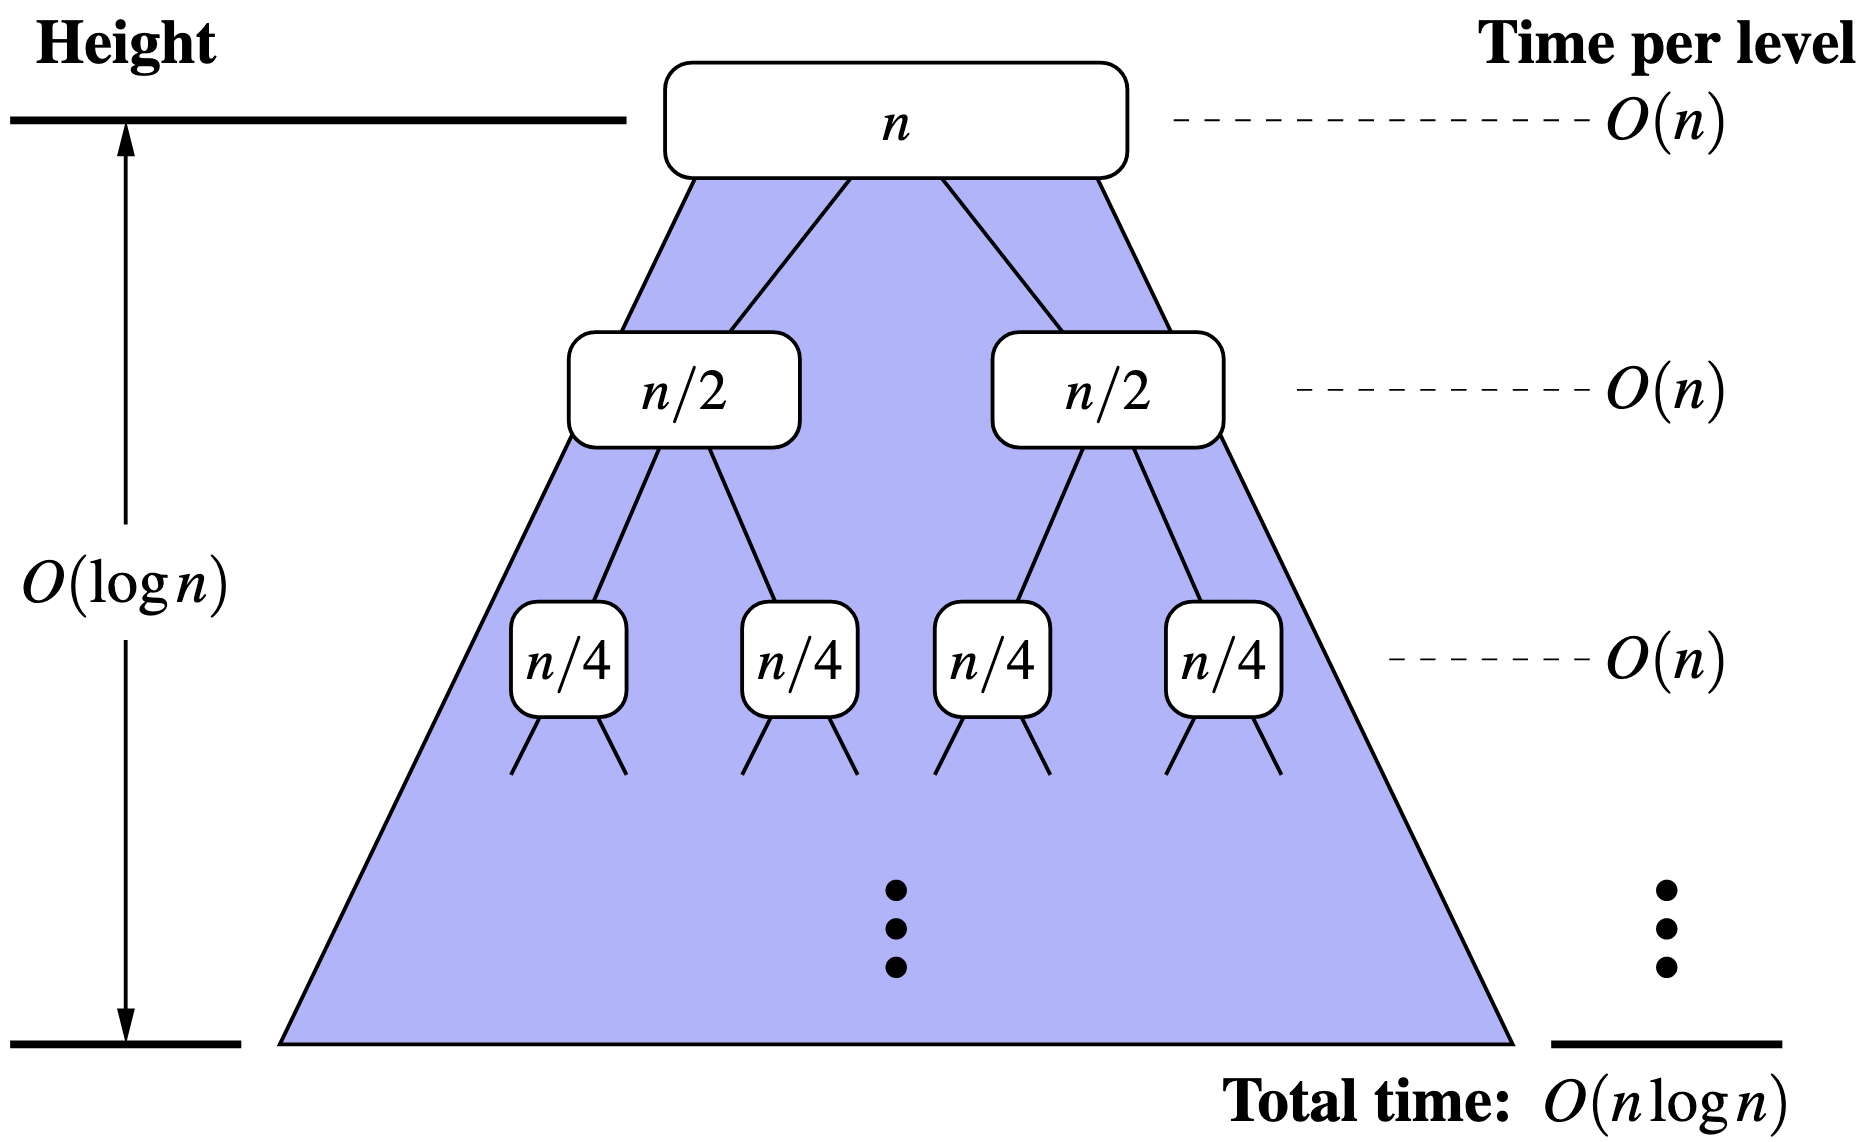
\includegraphics[scale=0.12]{graphic/05_laufzeit_mergesort} \\
                    \hline
                    Worst Case: $O(n*log(n))$ \\
                    Average Case: $O(n*log(n))$ \\
                    Best Case: $O(n*log(n))$ \\
                    \hline
                \end{tabular}

            \subsection{Quicksort}
                \begin{itemize}
                    \item Kein zusätzlicher Speicherbedarf
                \end{itemize}
                \begin{enumerate}
                    \item Pivot wählen
                    \item Array in 2 Unter-Arrays teilen $\to$ Elemente kleiner als Pivot und Elemente grösser als
                    Pivot
                    \item Quicksort rekursiv auf beiden Unter-Arrays aufrufen
                    \item Elemente des ersten Unter-Array, Pivot und Elemente des zweiten Unter-Arrays zurückgeben
                \end{enumerate}
                \begin{tabular}{|l|}
                    \hline
                    \textcolor{subsectioncolor}{Idee} \\
                    \begin{lstlisting}
                    def quicksort(array):
                        if len(array) < 2:
                            return array
                        else:
                            pivot = array[0]
                            less = [i for i in array[1:] if i <= pivot]
                            grater = [i for i in array[1:] if i > pivot]
                            return quicksort(less) + [pivot] + quicksort(greater)
                    \end{lstlisting} \\
                    \hline
                    \begin{lstlisting}
                    static void quickSort(int[] arr, int low, int high) {
                        if (low < high) {
                            int pi = partition(arr, low, high);
                            quicksort(arr, low, pi - 1);
                            quicksort(arr, pi + 1, high);
                        }
                    }
                    \end{lstlisting} \\
                    \hline
                    Worst Case: $O(n^2)$ \\
                    Average Case: $O(n*log(n))$ \\
                    Best Case: $O(n*log(n))$ \\
                    \hline
                \end{tabular}

            \section{Datenstruktur}
                \textcolor{subsectioncolor}{Beispiele für Datenstrukturen}
                \newline
                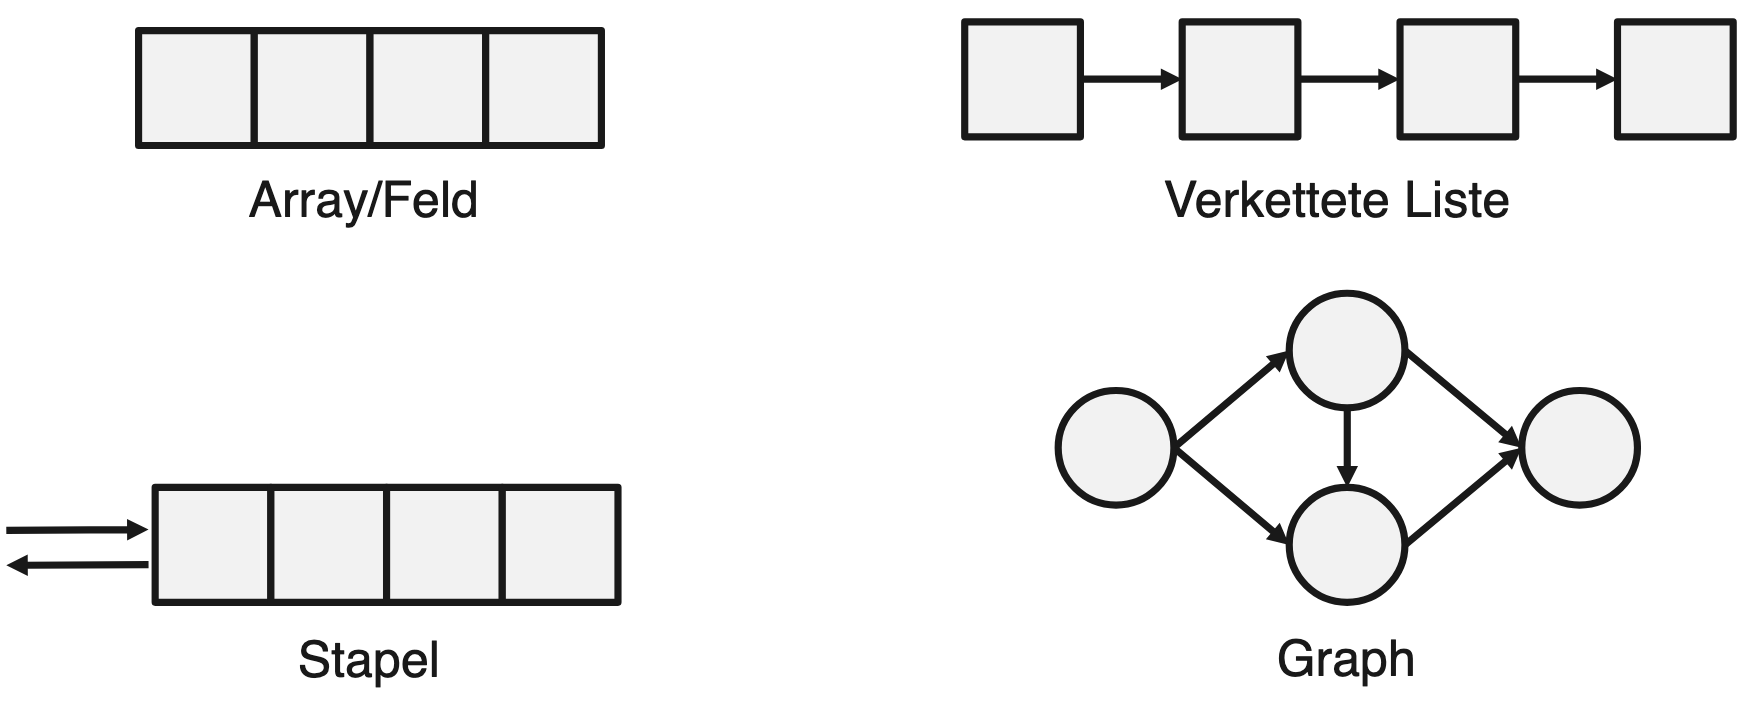
\includegraphics[scale=0.12]{graphic/06_adt_beispiele}

            \section{ADT (abstract data type)}
            Unterschied zur {\bfseries Datenstruktur}:
            \begin{itemize}
                \item abstrakter Datentyp (ADT) $\to$ eine Abstraktion einer konkreten Datenstruktur
                \item Datenstruktur $\to$ Realisierung / Implementierung eines ADT
                \item Datenstruktur $\to$ Speichern und organisieren Daten
            \end{itemize}
            \subsection{Definition}
                \begin{itemize}
                    \item ADT beschreibt
                    \begin{itemize}
                        \item Attribute
                        \item Operation auf Attributen
                        \item Ausnahmen und Fehler
                    \end{itemize}
                    \item Beschreibung des {\bfseries Was}, aber nicht des {\bfseries Wie}
                \end{itemize}

            \subsection{LinkedList<E>}
                \begin{tabular}{l|p{3cm}}
                    \texttt{void add(E item)} & item am Ende einfügen \\
                    \texttt{void add(int pos, E item)} & item an Position pos einfügen \\
                    \texttt{boolean contains(E item)} & Enthält Liste item? \\
                    \texttt{int size()} & Gibt Anzahl items in Liste zurück \\
                    \texttt{boolean isEmpty()} & Ist Liste leer? \\
                    \texttt{E get(int pos)} & Element an Position pos zurückgeben \\
                    \texttt{E remove(int pos)} & Element an Position pos entfernen und zurückgeben \\
                \end{tabular}
            
                \subsubsection{Doubly-Linked-List}
                    \begin{itemize}
                        \item Jeder Knoten speichert Verbindung zum Vorgänger \& Nachfolger
                        \item header \& trailer als Start-Knoten für Suche
                        \begin{itemize}
                            \item header \& trailer: Sentinels / Guards
                        \end{itemize}
                    \end{itemize}
                    \newline
                    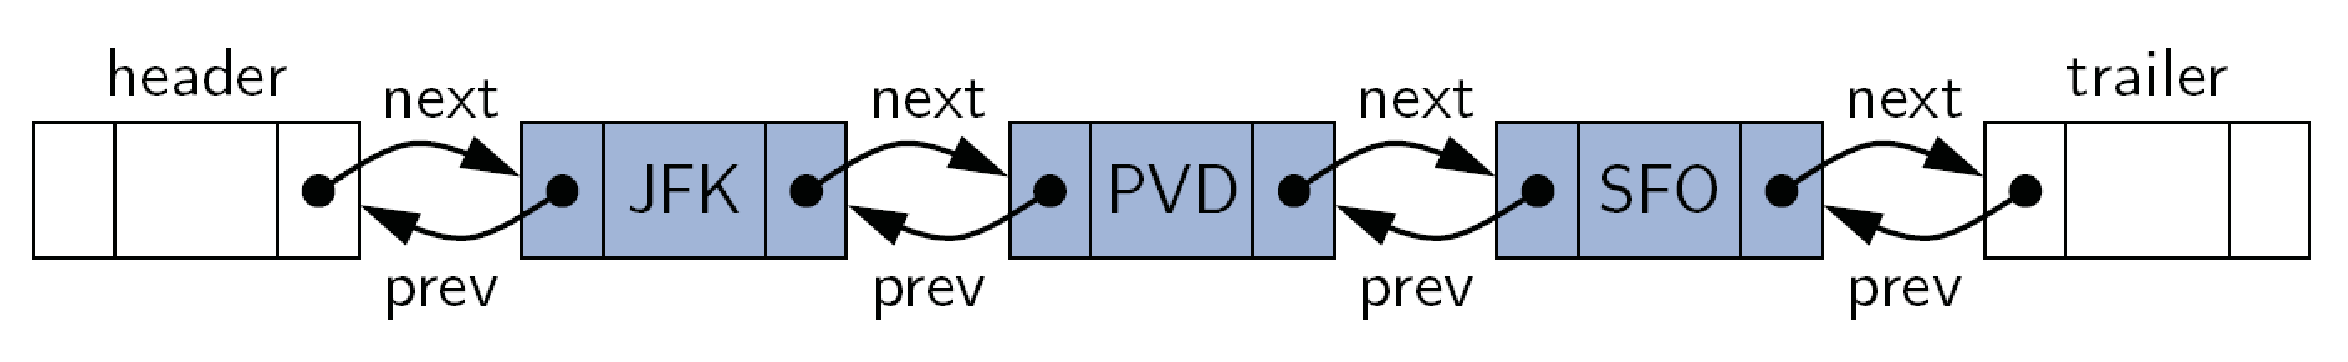
\includegraphics[scale=0.2,width=\columnwidth]{graphic/02_doubly-linkedlist}

        \subsection{Stack}
            \begin{itemize}
                \item Anwendung: Parser / Parsen von verschachtelten Klammern (())([()])
            \end{itemize}
            \newline
            \begin{lstlisting}
                    public interface Stack<E> {
                        int size();
                        boolean isEmpty();
                        void push(E element);
                        E top();
                        E pop();
                    }
            \end{lstlisting}
            \newline
            \newline
            \texttt{resize()} statt Exception
            \begin{lstlisting}
                    public void push(Item item) {
                        if (n == a.length) resize();
                        a[++n] = item;
                    }

                    private void resize() {
                        int oldSize = data.length;
                        int newSize = oldSize * RESIZE_FACTOR;

                        E[] temp = (E[]) new Object[newSize];
                        for (int i = 0; i < oldSize; i++) {
                            temp[i] = data[i];
                        }
                        data = temp;
                    }
            \end{lstlisting}
            \begin{lstlisting}
                    public class ArrayStack<E> implements Stack<E> {
                        private E[] data;
                        private int t = -1;

                        public ArrayStack(int capacity){
                            data = (E[]) new Object[capacity];
                        }

                        public int size() {
                            return (t + 1);
                        }

                        public boolean isEmpty(){
                            return (t == -1);

                        public void push(E element) throws IllegalStateException {
                            if (size() == data.length)
                                throw new IllegalStateException ("Stack is full!");
                            data[++t] = element;
                        }

                        public E top() {
                            if (isEmpty()) return null;
                                return data[t];
                        }

                        public E pop() {
                            if (isEmpty()) return null;
                            E element = data[t];
                            data[t--] = null;
                            return element;
                        }
                    }
            \end{lstlisting}

            \subsection{Queue}
                \begin{lstlisting}
                    public interface Queue<E> {
                        int size();
                        boolean isEmpty();
                        void enqueue(E element);
                        E first();
                        E dequeue();
                    }
                    ...
                    public void enqueue(E element) {
                        if (this.storedElements == this.capacity) {
                            throw new IllegalStateException();
                        } else {
                            int r = (this.frontElement + this.storedElements) % this.capacity;
                            this.data[r] = element;
                            this.storedElements++;
                        }
                    }
                    ...
                    public E dequeue() {
                        if (this.isEmpty()) {
                            return null;
                        } else {
                            E elem = this.data[this.frontElement];
                            this.frontElement = (this.frontElement + 1) % this.capacity;
                            this.storedElements--;
                            return elem;
                        }
                    }
                \end{lstlisting}

                %\subsubsection{Ringbuffer}

            \subsection{Priority Queue}
                \textcolor{subsectioncolor}{Entry und Priority Queue ADT}
                \begin{lstlisting}
                    public interface PriorityQueue<K, V> {
                        int size();
                        boolean isEmpty();
                        Entry<K, V> insert(K key, V value);
                        Entry<K, V> min();
                        Entry<K, V> removeMin();
                    }

                    public interface Entry<K,V> {
                        public K key();
                        public V value();
                    }
                \end{lstlisting}
                \textcolor{subsectioncolor}{Impl mit {\bfseries unsortierter} Liste: \texttt{insert()}}
                \begin{lstlisting}
                    @Override
                    public Entry<K,V> insert(K key, V value) {
                        checkKey(key);
                        Entry<K,V> newest = new PriorityQueueEntry<>(key, value);
                        list.add(newest);
                        return newest;
                    }
                \end{lstlisting}
                \textcolor{subsectioncolor}{Impl mit {\bfseries unsortierter} Liste: \texttt{removeMin()}}
                \textcolor{subsectioncolor}{Impl mit {\bfseries unsortierter} Liste: \texttt{removeMin()}}
                \begin{lstlisting}
                    @Override
                    public Entry<K,V> removeMin() {
                        if (list.isEmpty()) {
                            return null;
                        }
                        var entry = findMin();
                        list.remove(entry);
                        return entry;
                    }

                    private Entry<K,V> findMin() {
                        Entry<K,V> small = list.get(0);
                        for (Entry<K,V> walk : list) {
                            if (compare(walk, small) < 0) {
                                small = walk;
                            }
                        }
                        return small;
                    }
                \end{lstlisting}
                \textcolor{subsectioncolor}{Impl mit {\bfseries sortierter} Liste: \texttt{insert()}}
                \begin{lstlisting}
                    public Entry<K, V> insert(K key, V value) {
                        var newest = new PriorityQueueEntry<>(key, value);
                        if (list.size() == 0) {
                            list.add(newest);
                            return newest;
                        }
                        Entry<K,V> walk = list.get(list.size() - 1);
                        int index = 0;
                        for (index = list.size() - 1; index >= 0 && compare(newest, walk) > 0; index--) {
                            walk = list.get(index);
                        }
                        if (index == -1) {
                            list.add(newest);
                        } else {
                            list.add(index, newest);
                        }
                        return newest;
                    }
                \end{lstlisting}
                \textcolor{subsectioncolor}{Impl mit {\bfseries sortierter} Liste: \texttt{removeMin()}}
                \begin{lstlisting}
                    @Override
                    public Entry<K, V> removeMin() {
                        return list.remove(0);
                    }
                \end{lstlisting}
                \textcolor{subsectioncolor}{Priority Queue sortieren}
                \begin{lstlisting}
                    public static <E> void pqSort(ArrayList<E> sourceList, PriorityQueue<E, ?> pQueue) {
                        int n = sourceList.size();
                        for (int j = 0; j < n; j++) {
                            E element = sourceList.remove(0);
                            pQueue.insert(element, null);
                        }
                        for (int j = 0; j < n; j++) {
                            E element = pQueue.removeMin().getKey();
                            sourceList.add(element);
                        }
                    }
                \end{lstlisting}
                \textcolor{subsectioncolor}{Laufzeiten}
                \begin{tabular}{c|c|c}
                    {\bfseries Methode} & {\bfseries Unsorted List} & {\bfseries Sorted List} \\
                    \hline
                    {\bfseries size} & $O(1)$ & $O(1)$ \\
                    {\bfseries isEmpty} & $O(1)$ & $O(1)$ \\
                    {\bfseries insert} & $O(1)$ & $O(n)$ \\
                    {\bfseries min} & $O(n)$ & $O(1)$ \\
                    {\bfseries removeMin} & $O(n)$ & $O(1)$ \\
                \end{tabular}

        \section{Trees / Bäume}
            \begin{itemize}
                \item Zweidimensionale Datenstruktur
                \item Repräsentiert hierarchische Beziehungen
                \item Besteht aus\ldots
                \begin{itemize}
                    \item {\bfseries Knoten:} Objekte des Baums
                    \item {\bfseries Kanten:} Relationen zwischen Knoten
                \end{itemize}
            \end{itemize}
            \subsection{Terminologie}
                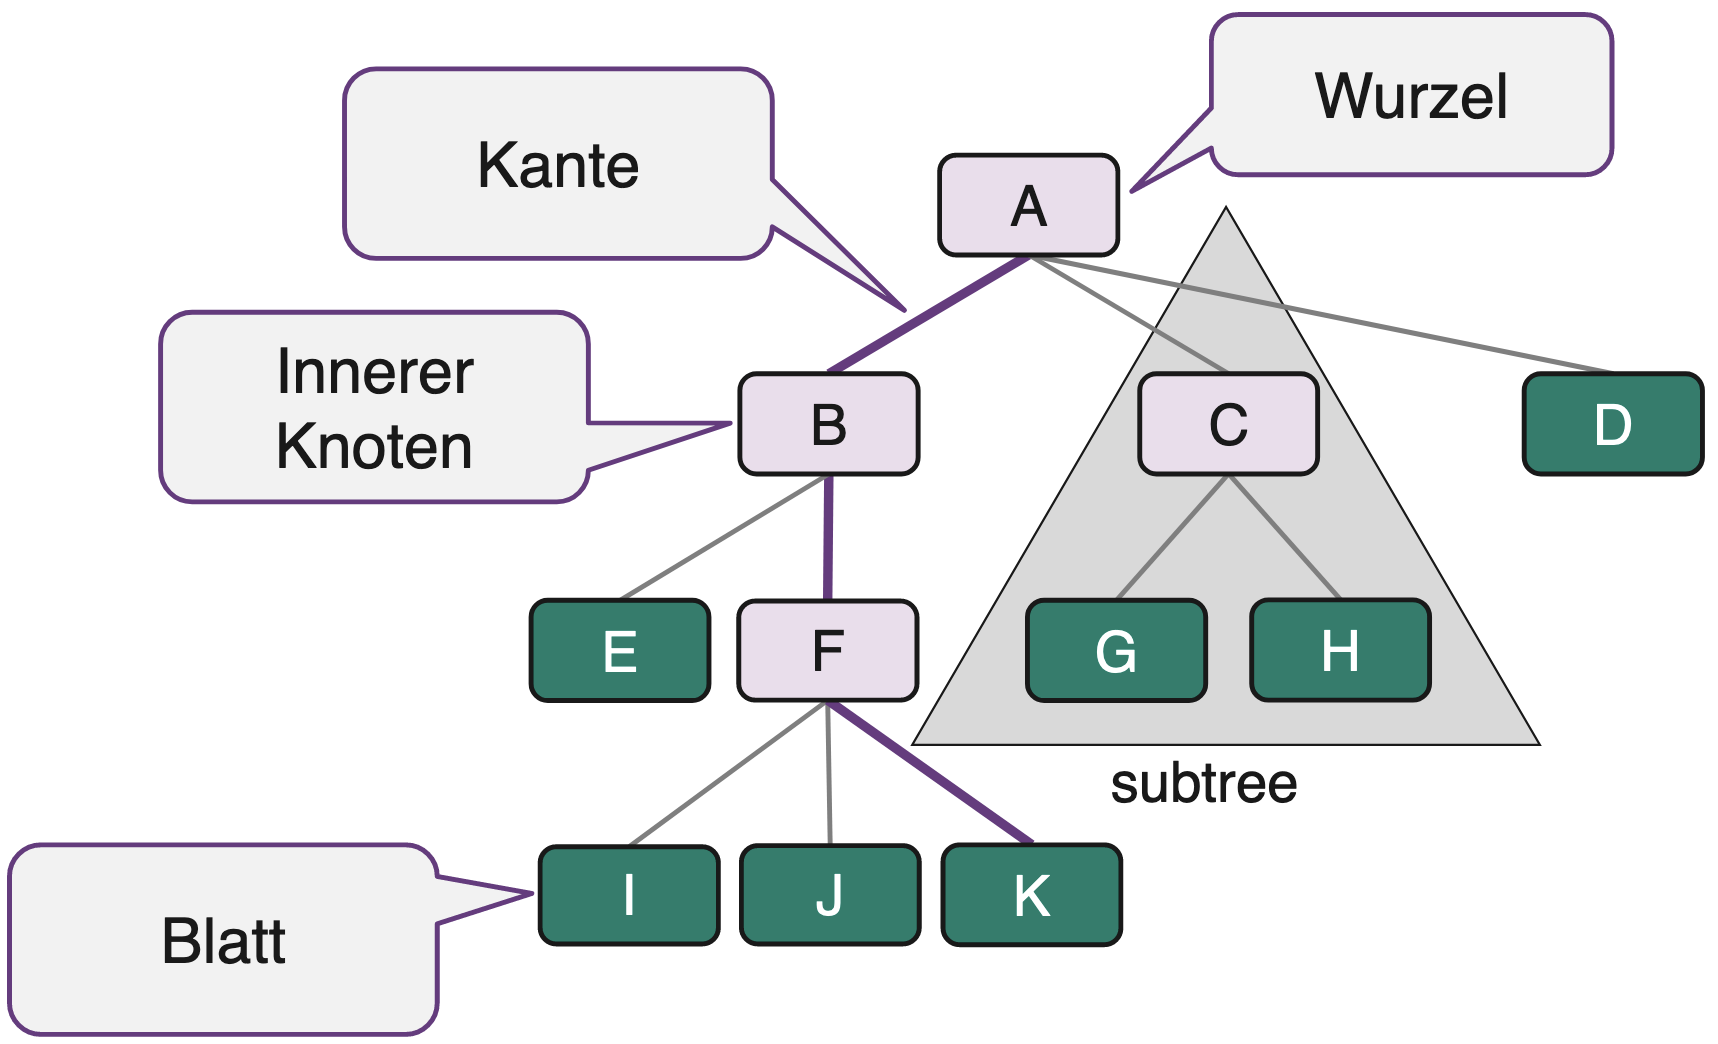
\includegraphics[scale=0.14]{graphic/09_terminologie_baum}
                \begin{itemize}
                    \item {\bfseries Wurzel:} Knoten ohne Elternknoten (A)
                    \item {\bfseries Innerer Knoten:} Knoten mit mind. einem Kind (A, B, C, F)
                    \item {\bfseries Blatt:} Knoten ohne Kinder (E, I, J, K, usw.)
                    \item {\bfseries Vorgängerknoten:} Eltern, Grosseltern, \ldots
                    \item {\bfseries Geschwister:} Knoten mit selben Eltern
                \end{itemize}

                \subsubsection{Tiefe}
                    \begin{itemize}
                        \item {\bfseries Tiefe} von $v$: \textcolor{subsectioncolor}{Vorfahren von $v$} (ohne $v$)
                    \end{itemize}
                    \textcolor{subsectioncolor}{Tiefe: Implementierung}
                    \begin{lstlisting}
                    public int depth(Position<E> p) {
                        if (isRoot(p)) {
                            return 0;
                        } else {
                            return 1 + depth(parent(p));
                        }
                    }
                    \end{lstlisting}

            \subsection{Binary Tree / Binärer Baum}
                \begin{itemize}
                    \item Innere Knoten: Höchstens 2 Kinder
                    \item Kinder eines Knotens sind geordnetes Paar (links, rechts)
                \end{itemize}
        
                \textcolor{subsectioncolor}{ADT in Java}
                \begin{lstlisting}
                    public interface BinaryTree<E> extends Tree<E> {
                        Position<E> left(Position<E> p);
                        Position<E> right(Position<E> p);
                        Position<E> sibling(Position<E> p);
                        Position<E> addRoot(E e);
                        Position<E> addLeft(Position<E> p, E e);
                        Position<E> addRight(Position<E> p, E e);
                    }
                \end{lstlisting}

            \subsection{Traversierungen}
                \begin{itemize}
                    \item Knoten systematisch besuchen
                    \item Algorithmen
                    \begin{itemize}
                        \item Preorder
                        \item Postorder
                        \item Breadth-First
                        \item Inorder
                    \end{itemize}
                \end{itemize}
        
                \subsubsection{Preorder (W-L-R)}
                    \begin{itemize}
                        \item Knoten wird {\bfseries vor} seinen Kindern besucht
                    \end{itemize}
                    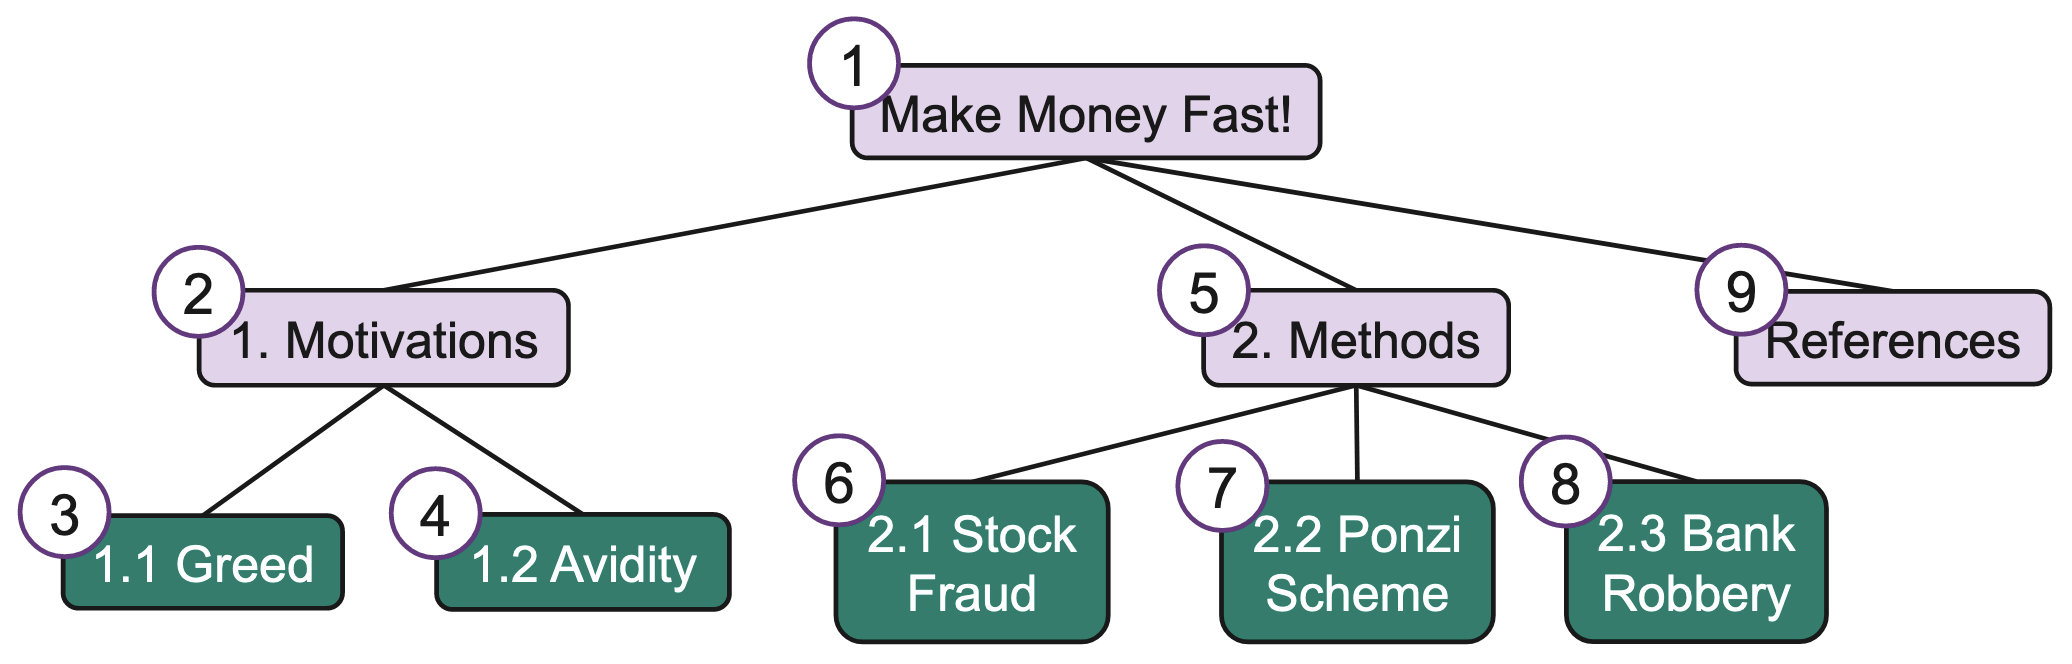
\includegraphics[scale=0.14]{graphic/10_baum_traversierung_preorder}
                    \begin{lstlisting}
                    algorithm preOrder(v)
                        visit(v)
                        for each child w of v
                            preOrder(w)
                    \end{lstlisting}
        
                \subsubsection{Postorder (L-R-W)}
                    \begin{itemize}
                        \item Knoten wird {\bfseries nach} seinen Nachfolgern besucht
                    \end{itemize}
                    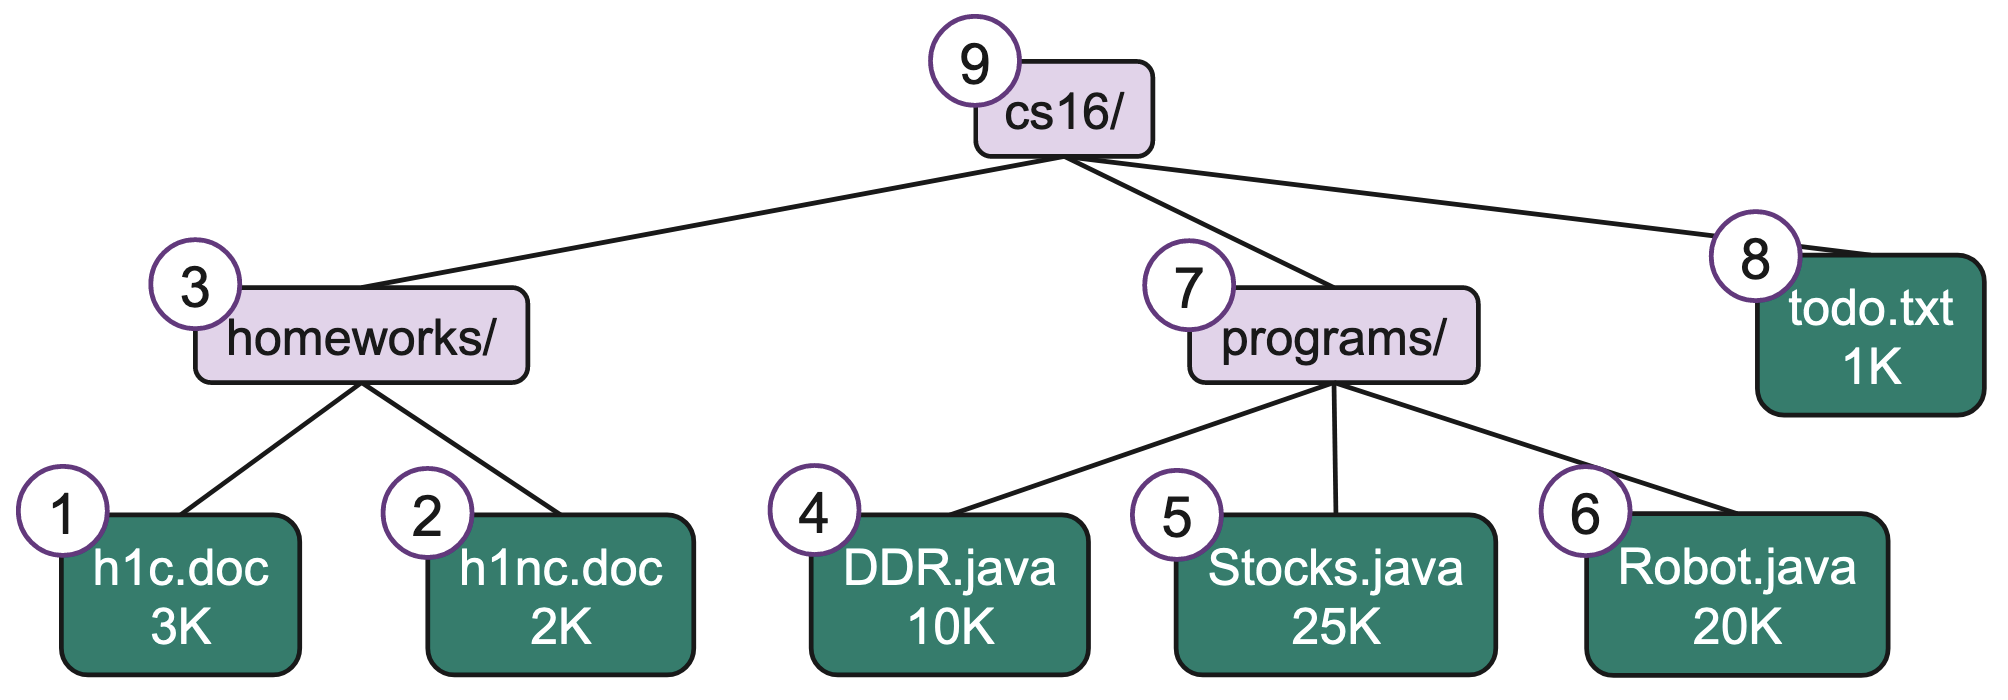
\includegraphics[scale=0.14]{graphic/11_baum_traversierung_postorder}
                    \begin{lstlisting}
                    algorithm postOrder(v)
                        for each child w of v
                            postOrder(w)
                        visit(v)
                    \end{lstlisting}
        
                \subsubsection{Breadth-First}
                    \begin{itemize}
                        \item {\bfseries Alle Knoten einer Stufe} besuchen, bevor Nachfolgeknoten besucht werden
                    \end{itemize}
                    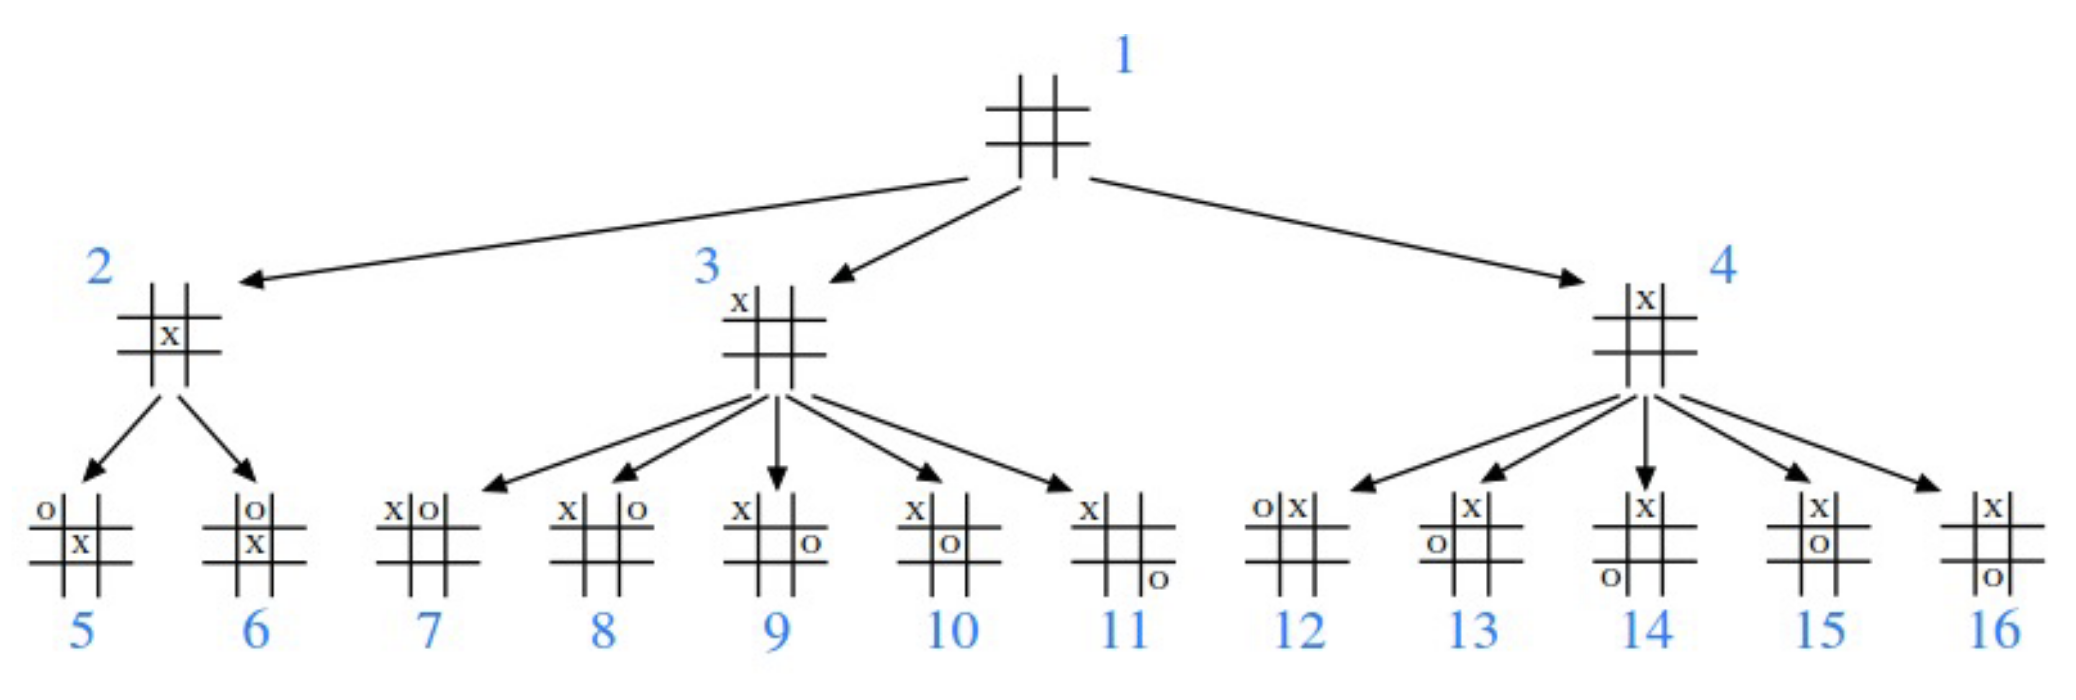
\includegraphics[scale=0.14]{graphic/12_baum_traversierung_breadth-first}
                    \begin{lstlisting}
                    Algorithm breadthFirst()
                    //Initialize queue Q containing root
                    while Q not empty
                        v = Q.dequeue()
                        visit(v)
                        for each child w in children(v)
                            Q.enqueue(w)
                    \end{lstlisting}
        
                \subsubsection{Inorder (L-W-R)}
                    \begin{itemize}
                        \item Knoten {\bfseries nach} linken Subtree und {\bfseries vor} rechtem Subtree besuchen
                        \item Darstellung von binären Bäumen
                        \begin{itemize}
                            \item $x(v)$ = inorder Rang von $v$
                            \item $y(v)$ = Tiefe von $v$
                        \end{itemize}
                    \end{itemize}
                    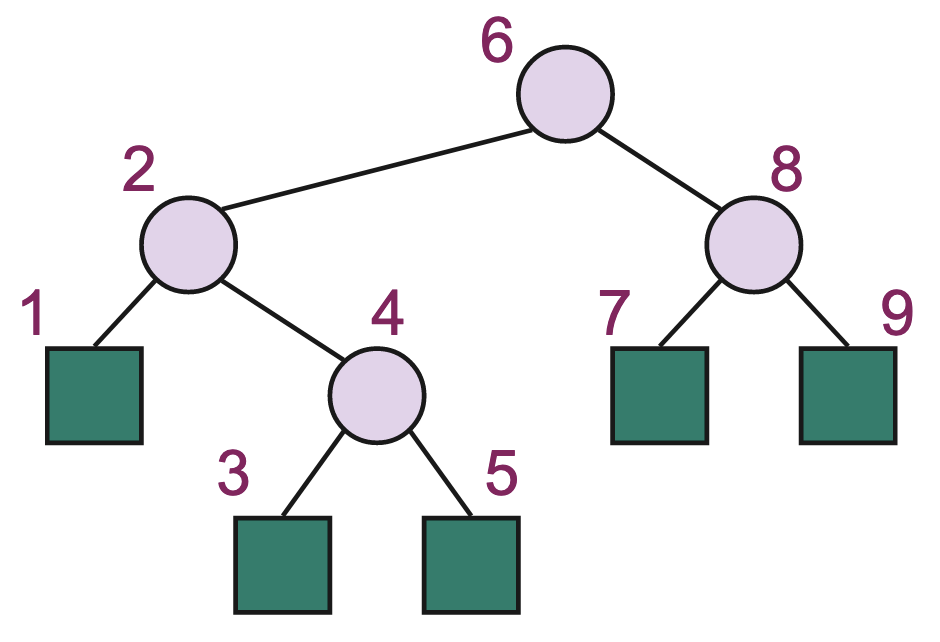
\includegraphics[scale=0.14]{graphic/13_baum_traversierung_inorder}
                    \begin{lstlisting}
                    algorithm inOrder(v)
                        if hasLeft(v)
                            inOrder(left(v))
                        visit(v)
                        if hasRight(v)
                            inOrder(right(v))
                    \end{lstlisting}


                \subsubsection{Auswertung von arithmetischen Ausdrücken / Euler-Tour}
                    \begin{lstlisting}
                    public int eulerPath(Node<E> node) {
                        Result result = new Result();
                        if (node == null) {
                            return 0;
                        }
                        if (node.isLeaf()) {
                            visitLeaf(node, result);
                        } else {
                            visitLeft(node, result);
                            result.leftResult = eulerPath(node.getLeft());
                            visitBelow(node, result);
                            result.rightResult = eulerPath(node.getRight());
                            visitRight(node, result);
                        }
                        return result.finalResult;
                    }
                    \end{lstlisting}

            \subsection{Heapsort}
                \begin{itemize}
                    \item Idee des Algorithmus
                    \begin{itemize}
                        \item Wurzel enthält immer kleinstes Element
                        \item Wiederholt Wurzelelement entnehmen bis Array leer ist
                    \end{itemize}
                \end{itemize}
                \subsubsection{Definition Heap}
                    \begin{itemize}
                        \item Binärer Baum mit folgenden Eigenschaften
                        \begin{itemize}
                            \item Baum ist vollständig
                            \item Schlüssel jedes Knoten kleiner oder gleich als Schlüssel seiner Kinder
                        \end{itemize}
                    \end{itemize}
                \subsubsection{Algorithmus}
                \begin{lstlisting}
                    algorithm HeapSort(F)
                        Eingabe: zu sortierende Folge F der Laenge n

                        Ueberfuehre F in Heap;
                        l := n; /* Letztes Element */
                        while l > 1 do
                            Vertausche F[1] und F[l];
                            Versenke F[1] im Heap F[1 ... l - 1];
                            l := l – 1
                        od
                \end{lstlisting}
                \subsubsection{Java Implementation}
                \begin{lstlisting}
                    public static void percolate(Comparable[] arrayToSort, int startIndex, int last) {
                        int i = startIndex;
                        while(hasLeftChild(i, last)) {
                            int leftChild = getLeftChild(i);
                            int rightChild = getRightChild(i);
                            int exchangeWith = 0;

                            if(arrayToSort[i].compareTo(arrayToSort[leftChild]) > 0) {
                                exchangeWith = leftChild;
                            }
                            if(rightChild <= last && arrayToSort[leftChild]
                                    .compareTo(arrayToSort[rightChild]) > 0) {
                                exchangeWith = rightChild;
                            }
                            if (exchangeWith == 0 || arrayToSort[i].compareTo(arrayToSort[exchangeWith]) <= 0) {
                                break;
                            }
                            swap(arrayToSort, i, exchangeWith);
                            i = exchangeWith;
                        }
                    }

                    public static void heapSort(Comparable[] arrayToSort) {
                        int i;
                        heapifyMe(arrayToSort);
                        for (i = arrayToSort.length - 1; i > 0; i--) {
                            swap(arrayToSort, 0, i); // Erstes Element mit letztem Tauschen
                            percolate(arrayToSort, 0, i - 1); // Heap wiederherstellen
                        }
                    }
                \end{lstlisting}

            \subsection{BinarySearchTree}
                \begin{lstlisting}
                    package ch.ost.oop.ex.task4;

                    import java.util.Iterator;
                    import java.util.List;
                    import java.util.Random;

                    import static java.lang.Math.max;

                    public class BinarySearchTree<E extends Comparable<E>> implements Iterable<E> {

                        private Node<E> root;

                        public void insertElement(E value) {
                            root = insertElement(value, root);
                        }

                        private Node<E> insertElement(E value, Node<E> node) {
                            if (node == null) {
                                node = new Node<>(value);
                            } else if (value.compareTo(node.getValue()) < 0) {
                                node.setLeft(insertElement(value, node.getLeft()));
                                if (getHeight(node.getLeft()) - getHeight(node.getRight()) == 2) {
                                    if (value.compareTo(node.getLeft().getValue()) < 0) {
                                        node = rotateWithLeftChild(node);
                                    } else {
                                        node = doubleWithLeftChild(node);
                                    }
                                }
                            } else if (value.compareTo(node.getValue()) > 0) {
                                node.setRight(insertElement(value, node.getRight()));
                                if (getHeight(node.getRight()) - getHeight(node.getLeft()) == 2) {
                                    if (value.compareTo(node.getRight().getValue()) > 0) {
                                        node = rotateWithRightChild(node);
                                    } else {
                                        node = doubleWithRightChild(node);
                                    }
                                }
                            }
                            node.setHeight(getMaxHeight(getHeight(node.getLeft()), getHeight(node.getRight())) + 1);

                            return node;

                        }

                        private Node<E> rotateWithLeftChild(Node<E> node2) {
                            Node<E> node1 = node2.getLeft();
                            node2.setLeft(node1.getRight());

                            node1.setRight(node2);

                            node2.setHeight(getMaxHeight(getHeight(node2.getLeft()), getHeight(node2.getRight())) + 1);
                            node1.setHeight(getMaxHeight(getHeight(node1.getLeft()), node2.getHeight()) + 1);

                            return node1;
                        }

                        private Node<E> rotateWithRightChild(Node<E> node1) {
                            Node<E> node2 = node1.getRight();
                            node1.setRight(node2.getLeft());

                            node2.setLeft(node1);

                            node1.setHeight(getMaxHeight(getHeight(node1.getLeft()), getHeight(node1.getRight())) + 1);
                            node2.setHeight(getMaxHeight(getHeight(node2.getRight()), node1.getHeight()) + 1);

                            return node2;
                        }

                        private Node<E> doubleWithLeftChild(Node<E> node3) {
                            node3.setLeft(rotateWithRightChild(node3.getLeft()));

                            return rotateWithLeftChild(node3);
                        }

                        private Node<E> doubleWithRightChild(Node<E> node1) {
                            node1.setRight(rotateWithLeftChild(node1.getRight()));

                            return rotateWithRightChild(node1);
                        }

                        private int getHeight(Node<E> node) {
                            return node == null ? -1 : node.getHeight();
                        }

                        private int getMaxHeight(int leftNodeHeight, int rightNodeHeight) {
                            return max(leftNodeHeight, rightNodeHeight);
                        }

                        public int size() {
                            return size(root);
                        }

                        private int size(Node<E> head) {
                            if (head == null) return 0;
                            else {
                                int length = 1;
                                length += size(head.getLeft());
                                length += size(head.getRight());
                                return length;
                            }
                        }

                        public Node<E> find(E value) {
                            Node<E> current = root;
                            while (current != null) {
                                if (current.getValue().compareTo(value) == 0) {
                                    break;
                                }
                                current = current.getValue().compareTo(value) < 0 ? current.getRight() : current.getLeft();
                            }
                            return current;
                        }

                        public Node<E> getRoot() {
                            return root;
                        }


                        @Override
                        public Iterator<E> iterator() {
                            return new TreeIteratorPreorder<>(root);
                        }


                        public static void main(String[] args) {

                            BinarySearchTree<Integer> bst = new BinarySearchTree<>();

                            List<Integer> list = List.of(21, 11, 5, 1, 0, 4, 9, 10, 13, 12, 18, 15, 20, 30, 25, 23, 22, 28, 43, 42, 34, 47, 44, 48);
                            for (Integer integer : list) {
                                bst.insertElement(integer);
                            }

                            for (Integer integer : bst) {
                                System.out.println(integer);
                            }
                        }

                    }
                \end{lstlisting}

                \subsubsection{Node}
                    \begin{lstlisting}
                    package ch.ost.oop.ex.task4;

                    class Node<E> {
                        private final E value;
                        private Node<E> left, right;
                        private int height;

                        public Node(E value) {
                            this.value = value;
                        }

                        public E getValue() {
                            return value;
                        }

                        public Node<E> getLeft() {
                            return left;
                        }

                        public void setLeft(Node<E> left) {
                            this.left = left;
                        }

                        public Node<E> getRight() {
                            return right;
                        }

                        public void setRight(Node<E> right) {
                            this.right = right;
                        }

                        public int getHeight() {
                            return height;
                        }

                        public void setHeight(int height) {
                            this.height = height;
                        }
                    }
                    \end{lstlisting}
                
                \subsubsection{TreeIteratorPreorder}
                    \begin{lstlisting}
                    package ch.ost.oop.ex.task4;

                    import java.util.Iterator;
                    import java.util.Stack;

                    public class TreeIteratorPreorder<T> implements Iterator<T> {

                        private Node<T> root;
                        private final Stack<Node<T>> visiting;

                        public TreeIteratorPreorder(Node<T> root) {
                            visiting = new Stack<>();
                            this.root = root;
                        }

                        @Override
                        public boolean hasNext() {
                            return root != null;
                        }

                        @Override
                        public T next() {
                            if (visiting.empty()) {
                                visiting.push(root);
                            }
                            Node<T> node = visiting.pop();

                            if (node.getRight() != null) {
                                visiting.push(node.getRight());
                            }
                            if (node.getLeft() != null) {
                                visiting.push(node.getLeft());
                            }

                            if (visiting.empty()) {
                                root = null;
                            }
                            return node.getValue();
                        }
                    }
                    \end{lstlisting}

        %\section{Design Patterns}
        %    \subsection{Iterator}
        %    \subsection{Adapter}
        %    \subsection{Visitor}
        %    \subsection{Template}

        \section{Hashing}
            \textcolor{subsectioncolor}{Eigenschaften guter Hashfunktionen}
            \begin{itemize}
                \item Konsistenz (gleicher Input $\to$ gleicher Output)
                \item Effiziente Berechnung
                \item Gleichmässige Verteilung der Schlüssel
            \end{itemize}

            \subsection{Integer Cast}
                \begin{itemize}
                    \item Gut $\to$ Anzahl bits erlaubt Interpretation als Integer
                    \item Schlecht $\to$ Schlüssel ist länger
                \end{itemize}

            \subsection{Komponentensumme}
                \begin{itemize}
                    \item Bits des Keys in Komponenten fixer länge (16/32 bits) unterteilen
                    \begin{itemize}
                        \item Komponenten summieren, Overflow ignorieren
                    \end{itemize}
                    \item Gut für Schlüssel fixer Länge, $>=$ Anzahl bits von Integer
                \end{itemize}

            \subsection{Polynom-Akkumulation}
                \begin{itemize}
                    \item Hashing von Werten der Form $(x_0, x_1, \dots, x_{n-1})$
                    \item Polynom
                    \begin{itemize}
                        \item $p(z) = a_0 + a_1 z + a_2 z^2 + \dots + a_{n-1} z^{n-1}$
                        \item für fixes $z$
                    \end{itemize}
                    \item Gut für Strings
                    \begin{itemize}
                        \item Mit $z = 33$ max. 6 Kollisionen bei 50.000 englischen Wörtern
                    \end{itemize}
                    \item \texttt{String.hashCode()}
                    \begin{itemize}
                        \item \begin{lstlisting}
                    s[0] * 31 ^ (n - 1) + s[1] * 31 ^ (n - 2) + ... + s[n - 1]
                        \end{lstlisting}
                    \end{itemize}
                \end{itemize}

            \subsection{Kollisionen (inkl. Behandlung)}
                \subsubsection{Geschlossene Addressierung}
                    \begin{itemize}
                        \item Behälter sind (verkettete) Listen
                        \item Platz nicht begrenzt, prinzipiell keine Überläufer
                    \end{itemize}
                    \textcolor{subsectioncolor}{Separate Chaining}
                    \begin{itemize}
                        \item Jede Zelle der Tabelle zeigt auf Liste
                        \item Gut: Einfach
                        \item Schlecht: Zusätzliche Datenstruktur und Speicherbedarf
                        \item Lineare Suche im Bucket: $O\frac{n}{N}$, $n =$ Einträge in Tabelle, $N =$ Buckets
                    \end{itemize}

                \subsubsection{Offene Addressierung}
                    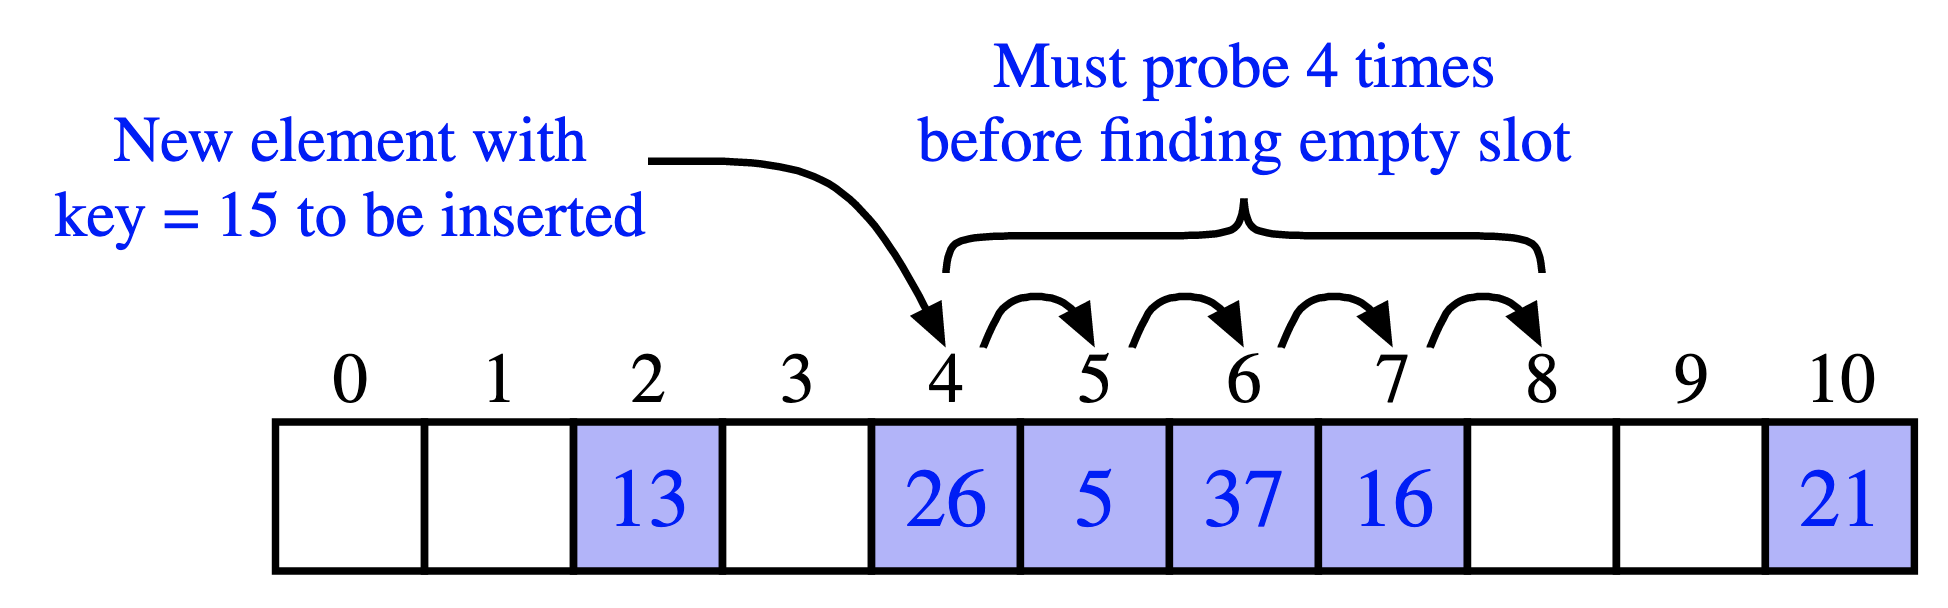
\includegraphics[scale=0.15]{graphic/17_hashing_offene_addressierung}
                    \begin{itemize}
                        \item Für Überläufer in anderen Behältern Platz suchen (Sondierung)
                        \item Sondierungsfolge bestimmt Weg zum Speichern \& Finden der Überläufer
                        \item erfordert besondere Behandlung der Lösch-Operationen
                        \item Wird element gelöscht, kann Sondierungsfolge für anderen Datensatz unterbrechen
                        \item Beim Sondieren werden Behälter mit gelöschten Datensätzen wie belegte Behälter zum
                        weiterhangeln benutzt
                    \end{itemize}
        
                \subsubsection{Konsistentes Hashing}
                    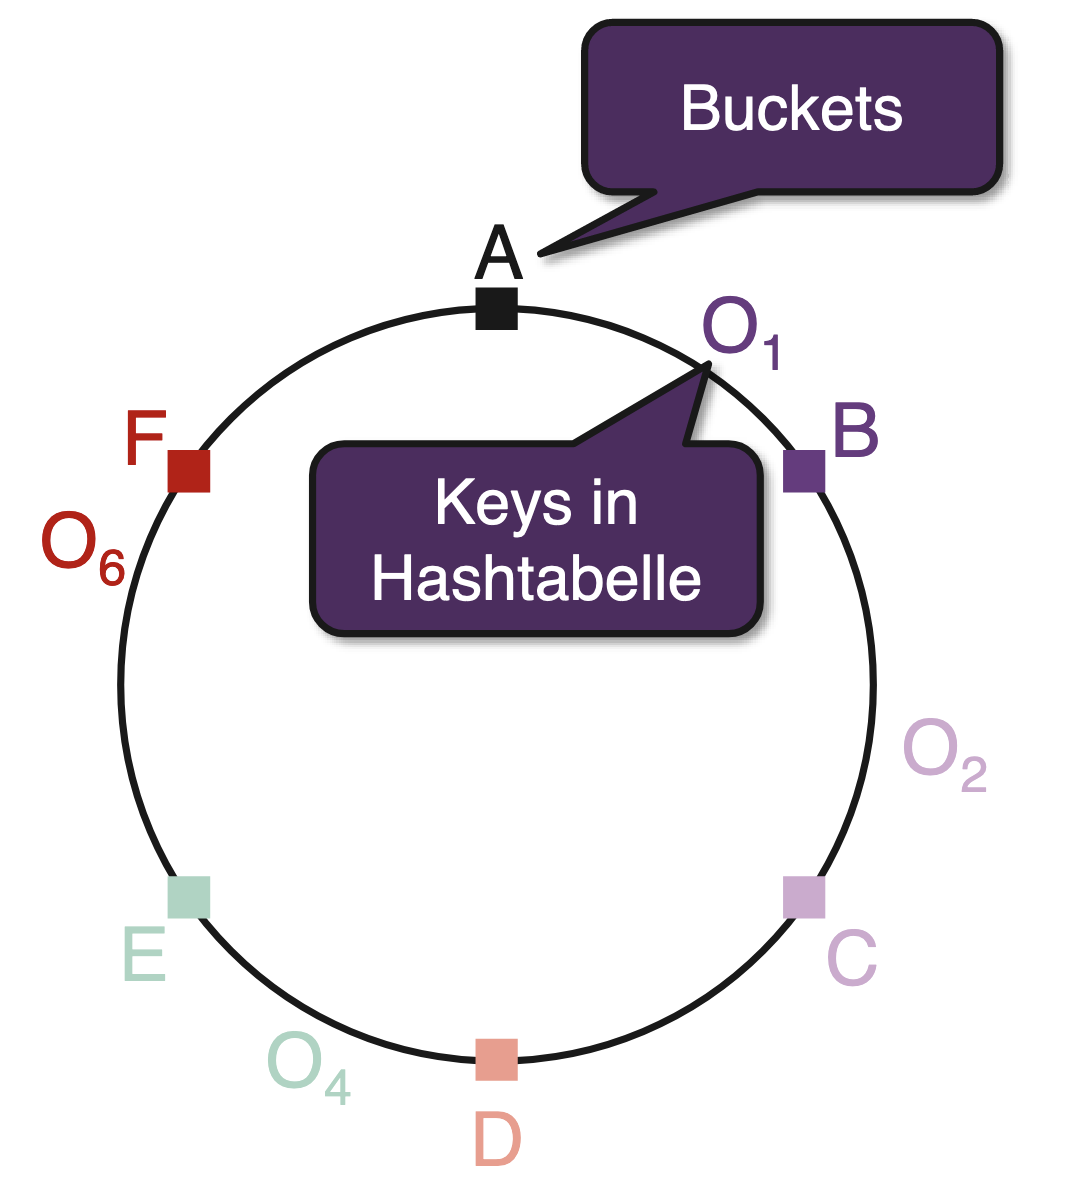
\includegraphics[scale=0.15]{graphic/16_konsistentes_hashing_ring}
                    \begin{itemize}
                        \item Keys werden auf Ring angeordnet
                        \item im Uhrzeigersinn werden Keys dem nächsten Bucket zugeordnet
                        \item Änderungen wirken sich nur auf direkte Nachbarn aus
                    \end{itemize}
        
            \subsection{Hashing in Java}
                \begin{itemize}
                    \item Wenn für Klasse \texttt{equals()} überschrieben wird muss auch \texttt{hashCode()}
                    überschrieben werden
                \end{itemize}
                \textcolor{subsectioncolor}{IntelliJ IDEA Standard \texttt{hashCode()} Implementierung}
                \begin{lstlisting}
                    @Override
                    public int hashCode() {
                        int result = (int) (id ^ (id >>> 32));
                        result = 31 * result + name.hashCode();
                        result = 31 * result + email.hashCode();
                        return result;
                    }
                \end{lstlisting}
                \subsubsection{Gleichheit}
                    \begin{itemize}
                        \item Referenzvergleich: \texttt{equals()} standardmässig Referenzvergleich
                        (referential equality)
                        \begin{itemize}
                            \item \texttt{a.equals(b)} vs \texttt{a == b}
                        \end{itemize}
                        \item Inhaltsvergleich: \texttt{equals()} überschreiben (structural equality)
                        \begin{itemize}
                            \item Bei String implementiert (bei anderen Datentypen nicht!)
                        \end{itemize}
                    \end{itemize}

        \section{Maps}
            \subsection{Map mit Unsortierter Liste}
                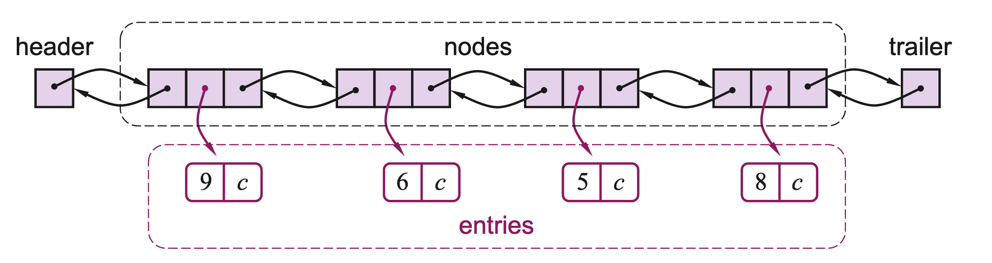
\includegraphics[scale=0.16]{graphic/18_map_mit_unsortierter_liste}

                \subsubsection{Get}
                    \begin{lstlisting}
                    public V get(K key) {
                        var iter = this.list.iterator();
                        while (iter.hasNext()) {
                            var node = iter.next();
                            if (node.getKey().equals(key)) {
                                return node.getValue();
                            }
                        }
                        return null;
                    }
                    \end{lstlisting}
                
                \subsubsection{Put}
                    \begin{lstlisting}
                    public V put(K key, V value) {
                        var iter = this.list.iterator();
                        while (iter.hasNext()) {
                            var node = iter.next();
                            if (node.getKey().equals(key)) {
                                V t = node.getValue();
                                node.setValue(value);
                                return t;
                            }
                        }
                        this.list.addLast(new ListNode<K, V>(key, value));
                        return null;
                    }
                    \end{lstlisting}

                \subsubsection{Remove}
                    \begin{lstlisting}
                    public V remove(K key) {
                    var iter = this.list.iterator();
                        while (iter.hasNext()) {
                            var node = iter.next();
                            if (node.getKey().equals(key)) {
                                V val = node.getValue();
                                list.remove(node);
                                return val;
                            }
                        }
                        return null;
                    }
                    \end{lstlisting}

            \subsection{Multimap}
                \begin{itemize}
                    \item Ähnlich aufgebaut wie Map: speichert <k, v>-Paare
                    \item Multimap kann zu Schlüssel k mehrere Einträge aufnehmen
                    \begin{itemize}
                        \item <k, v> und <k, v'>
                        \begin{itemize}
                            \item Schloss $\to$ Gebäude
                            \item Schloss $\to$ Verriegelung
                        \end{itemize}
                    \end{itemize}
                    \item Lösungsansatz
                    \begin{itemize}
                        \item Ansatz 1: Anpassen der Datenstruktur
                        \item Ansatz 2: Schlüssel k verweist auf Collection mit Werten k
                    \end{itemize}
                \end{itemize}

                \subsubsection{Interface}
                    \begin{lstlisting}
                    package ch.ost.oop2.hashmultimap;
                    import java.util.Map;

                    public interface Multimap<K, V> {
                        public Iterable<V> get (K key);
                        public void put(K key, V value);
                        public boolean remove(K key, V value);
                        public Iterable<V> removeAll(K key);
                        public Iterable<Map.Entry<K, V>> entries();
                        public int size();
                        public boolean isEmpty();
                    }
                    \end{lstlisting}
                \subsubsection{Multimap Impl}
                    \begin{lstlisting}
                    public class HashMultimap<K, V> implements Multimap<K, V> {
                        Map <K, List<V>> map = new HashMap<>();

                        int numberOfEntries = 0;
                        public HashMultimap() {};

                        @Override
                        public int size() {
                            return numberOfEntries;
                        }

                        @Override
                        public boolean isEmpty() {
                            return (numberOfEntries == 0);
                        }
                        // ...
                    }
                    \end{lstlisting}
                \subsubsection{Put}
                    \begin{lstlisting}
                    @Override
                    public void put(K key, V value) {
                        List<V> secondary = map.get(key);
                        if (secondary == null) {
                            secondary = new ArrayList<>();
                            map.put(key, secondary);
                        }
                        secondary.add(value);
                        numberOfEntries++;
                    }
                    \end{lstlisting}
                \subsubsection{Get}
                    \begin{lstlisting}
                    @Override
                    public Iterable<V> get (K key) {
                        List<V> secondary = map.get(key);
                        if (secondary != null) {
                            return secondary;
                        }
                        return new ArrayList<>();
                    }
                    \end{lstlisting}
                \subsubsection{Remove}
                    \begin{lstlisting}
                    @Override
                    public boolean remove(K key, V value) {
                        boolean wasRemoved = false;
                        List<V> secondary = map.get(key);
                        if (secondary != null) {
                            wasRemoved = secondary.remove(value);
                            if (wasRemoved) {
                                numberOfEntries--;
                                if(secondary.isEmpty()) {
                                    map.remove(key);
                                }
                            }
                        }
                        return wasRemoved;
                    }
                    \end{lstlisting}

            \subsection{SeparateChainingMap}
                \begin{lstlisting}
                    package ch.ost.oop.ex12.task1;
                    import java.util.*;

                    public class SeparatChainingMap<K, V> {
                        List<Entry<K, V>> entries;
                        int maxSize;
                        int size;

                        public SeparatChainingMap() {
                            maxSize = 10;
                            this.entries = new ArrayList<>();
                            for (int i = 0; i < maxSize; i++) {
                                entries.add(null);
                            }
                        }

                        private int getListIndex(K key) {
                            return Math.abs(Objects.hashCode(key) % maxSize);
                        }

                        public V get(K key) {
                            Entry<K, V> entry = getEntry(key);
                            if (entry == null) {
                                return null;
                            }
                            return entry.getValue();
                        }

                        private Entry<K, V> getEntry(K key) {
                            int index = getListIndex(key);
                            Entry<K, V> current = entries.get(index);
                            while (current != null) {
                                if (current.getKey().equals(key)) {
                                    return current;
                                }
                                current = current.getNext();
                            }

                            return null;
                        }

                        public V put(K key, V value) {
                            int index = getListIndex(key);
                            Entry<K, V> newEntry = new Entry<>(key, value);
                            Entry<K, V> current = entries.get(index);
                            if (current == null) {
                                entries.set(index, newEntry);
                                size++;
                            } else {
                                while (current != null) {
                                    if (current.getKey().equals(key)) {
                                        V before = current.getValue();
                                        current.setValue(value);
                                        expandTable();
                                        return before;
                                    }
                                    current = current.getNext();
                                }
                                current = entries.get(index);
                                newEntry.setNext(current);
                                entries.set(index, newEntry);
                                size++;
                            }
                            expandTable();
                            return null;
                        }

                        private void expandTable() {
                            if (1.0d * size / maxSize > 0.7) {
                                List<Entry<K, V>> tmp = entries;
                                entries = new ArrayList<>();
                                maxSize *= 2;
                                for (int i = 0; i < maxSize; i++) {
                                    entries.add(null);
                                }
                                for (Entry<K, V> entry : tmp) {
                                    while (entry != null) {
                                        put(entry.getKey(), entry.getValue());
                                        entry = entry.getNext();
                                    }
                                }
                            }
                        }

                        public V remove(K key) {
                            int index = getListIndex(key);
                            Entry<K, V> current = entries.get(index);
                            if (current == null) {
                                return null;
                            }
                            if (current.getKey().equals(key)) {
                                V val = current.getValue();
                                current = current.getNext();
                                entries.set(index, current);
                                size--;
                                return val;
                            } else {
                                Entry<K, V> prev = null;
                                while (current != null) {

                                    if (current.getKey().equals(key)) {
                                        prev.setNext(current.getNext());
                                        size--;
                                        return current.getValue();
                                    }
                                    prev = current;
                                    current = current.getNext();
                                }
                                return null;
                            }
                        }

                        public int size() {
                            return size;
                        }

                        public boolean isEmpty() {
                            return size == 0;
                        }

                        public Set<K> keySet() {
                            Set<K> set = new HashSet<>();
                            for (Entry<K, V> entry : entries) {
                                if (entry != null) {
                                    Entry<K, V> current = entry;
                                    while (current != null) {
                                        set.add(current.getKey());
                                        current = current.getNext();
                                    }
                                }
                            }
                            return set;
                        }

                        public Collection<V> values() {
                            List<V> list = new ArrayList<>();
                            for (Entry<K, V> entry : entries) {
                                if (entry != null) {
                                    Entry<K, V> current = entry;
                                    while (current != null) {
                                        list.add(current.getValue());
                                        current = current.getNext();
                                    }
                                }
                            }
                            return list;
                        }

                        public Collection<Entry<K, V>> entrySet() {
                            List<Entry<K, V>> list = new ArrayList<>();
                            for (Entry<K, V> entry : entries) {
                                if (entry != null) {
                                    Entry<K, V> current = entry;
                                    while (current != null) {
                                        list.add(current);
                                        current = current.getNext();
                                    }
                                }
                            }
                            return list;
                        }

                        public void print() {
                            for (Entry<K, V> entry : entries) {
                                if (entry == null) {
                                    System.out.println("null");
                                    continue;
                                }
                                while (entry != null) {
                                    System.out.print(entry);
                                    System.out.print(" --> ");
                                    entry = entry.getNext();
                                }
                                System.out.println();
                            }
                        }
                    }
                \end{lstlisting}
                \subsubsection{Entry}
                    \begin{lstlisting}
                    package ch.ost.oop.ex12.task1;
                    import java.util.Objects;

                    public class Entry<K, V> {
                        private final K key;
                        private V value;
                        private Entry<K, V> next;

                        public Entry(K key, V value) {
                            this.key = key;
                            this.value = value;
                        }

                        public K getKey() {
                            return key;
                        }

                        public V getValue() {
                            return value;
                        }

                        public void setValue(V value) {
                            this.value = value;
                        }

                        public Entry<K, V> getNext() {
                            return next;
                        }

                        public void setNext(Entry<K, V> next) {
                            this.next = next;
                        }

                        @Override
                        public String toString() {
                            return "Entry{" +
                                    "key=" + key +
                                    ", value=" + value +
                                    '}';
                        }

                        @Override
                        public boolean equals(Object o) {
                            if (this == o) return true;
                            if (o == null || getClass() != o.getClass()) return false;
                            Entry<?, ?> entry = (Entry<?, ?>) o;
                            return Objects.equals(key, entry.key) && Objects.equals(value, entry.value);
                        }

                        @Override
                        public int hashCode() {
                            return Objects.hash(key, value);
                        }
                    }
                    \end{lstlisting}

    \end{multicols*}

\end{document}